\documentclass[a4paper,12pt,twoside]{report}
\usepackage[left=3cm,right=3cm,top=3cm,bottom=3cm]{geometry} %Margins
\usepackage{pdfpages}
\usepackage{hyperref}
\usepackage{listings}
\usepackage{xcolor}
\usepackage{setspace}
\usepackage{tocloft}
\usepackage{amsmath}
\usepackage{chngcntr }
\usepackage[toc,page]{appendix}
\usepackage[T1]{fontenc}
\usepackage[nottoc]{tocbibind}
\usepackage[compact]{titlesec}
\titlespacing{\section}{0pt}{1ex}{0ex}
\titlespacing{\subsection}{0pt}{1ex}{0ex}
\titlespacing{\subsubsection}{0pt}{1ex}{0ex}

\counterwithout{figure}{chapter}
\counterwithout{table}{chapter}

\usepackage{graphicx}
\usepackage{verbatim}
\usepackage{latexsym}
\def\bbbr{{\rm I\!R}} %reelle Zahlen
\def\bbbm{{\rm I\!M}}
\def\bbbn{{\rm I\!N}} %natuerliche Zahlen
\def\bbbf{{\rm I\!F}}
\def\bbbh{{\rm I\!H}}
\def\bbbk{{\rm I\!K}}
\def\bbbp{{\rm I\!P}}
\def\bbbe{{\rm I\!E}}
\def\bbbone{{\mathchoice {\rm 1\mskip-4mu l} {\rm 1\mskip-4mu l}
{\rm 1\mskip-4.5mu l} {\rm 1\mskip-5mu l}}}
\def\bbbc{{\mathchoice {\setbox0=\hbox{$\displaystyle\rm C$}\hbox{\hbox
to0pt{\kern0.4\wd0\vrule height0.9\ht0\hss}\box0}}
{\setbox0=\hbox{$\textstyle\rm C$}\hbox{\hbox
to0pt{\kern0.4\wd0\vrule height0.9\ht0\hss}\box0}}
{\setbox0=\hbox{$\scriptstyle\rm C$}\hbox{\hbox
to0pt{\kern0.4\wd0\vrule height0.9\ht0\hss}\box0}}
{\setbox0=\hbox{$\scriptscriptstyle\rm C$}\hbox{\hbox
to0pt{\kern0.4\wd0\vrule height0.9\ht0\hss}\box0}}}}
\def\bbbq{{\mathchoice {\setbox0=\hbox{$\displaystyle\rm
Q$}\hbox{\raise
0.15\ht0\hbox to0pt{\kern0.4\wd0\vrule height0.8\ht0\hss}\box0}}
{\setbox0=\hbox{$\textstyle\rm Q$}\hbox{\raise
0.15\ht0\hbox to0pt{\kern0.4\wd0\vrule height0.8\ht0\hss}\box0}}
{\setbox0=\hbox{$\scriptstyle\rm Q$}\hbox{\raise
0.15\ht0\hbox to0pt{\kern0.4\wd0\vrule height0.7\ht0\hss}\box0}}
{\setbox0=\hbox{$\scriptscriptstyle\rm Q$}\hbox{\raise
0.15\ht0\hbox to0pt{\kern0.4\wd0\vrule height0.7\ht0\hss}\box0}}}}
\def\bbbt{{\mathchoice {\setbox0=\hbox{$\displaystyle\rm
T$}\hbox{\hbox to0pt{\kern0.3\wd0\vrule height0.9\ht0\hss}\box0}}
{\setbox0=\hbox{$\textstyle\rm T$}\hbox{\hbox
to0pt{\kern0.3\wd0\vrule height0.9\ht0\hss}\box0}}
{\setbox0=\hbox{$\scriptstyle\rm T$}\hbox{\hbox
to0pt{\kern0.3\wd0\vrule height0.9\ht0\hss}\box0}}
{\setbox0=\hbox{$\scriptscriptstyle\rm T$}\hbox{\hbox
to0pt{\kern0.3\wd0\vrule height0.9\ht0\hss}\box0}}}}
\def\bbbs{{\mathchoice
{\setbox0=\hbox{$\displaystyle     \rm S$}\hbox{\raise0.5\ht0\hbox
to0pt{\kern0.35\wd0\vrule height0.45\ht0\hss}\hbox
to0pt{\kern0.55\wd0\vrule height0.5\ht0\hss}\box0}}
{\setbox0=\hbox{$\textstyle        \rm S$}\hbox{\raise0.5\ht0\hbox
to0pt{\kern0.35\wd0\vrule height0.45\ht0\hss}\hbox
to0pt{\kern0.55\wd0\vrule height0.5\ht0\hss}\box0}}
{\setbox0=\hbox{$\scriptstyle      \rm S$}\hbox{\raise0.5\ht0\hbox
to0pt{\kern0.35\wd0\vrule height0.45\ht0\hss}\raise0.05\ht0\hbox
to0pt{\kern0.5\wd0\vrule height0.45\ht0\hss}\box0}}
{\setbox0=\hbox{$\scriptscriptstyle\rm S$}\hbox{\raise0.5\ht0\hbox
to0pt{\kern0.4\wd0\vrule height0.45\ht0\hss}\raise0.05\ht0\hbox
to0pt{\kern0.55\wd0\vrule height0.45\ht0\hss}\box0}}}}
\def\bbbz{{\mathchoice {\hbox{$\mathsf\textstyle Z\kern-0.4em Z$}}
{\hbox{$\mathsf\textstyle Z\kern-0.4em Z$}}
{\hbox{$\mathsf\scriptstyle Z\kern-0.3em Z$}}
{\hbox{$\mathsf\scriptscriptstyle Z\kern-0.2em Z$}}}}
\usepackage{setspace}
\usepackage{blindtext}
\usepackage{float}
\usepackage{amsmath}

\setlength{\parskip}{\medskipamount}  % a little space before a \par
\setlength{\parindent}{0pt}	      % don't indent first lines of paragraphs
%UHEAD.STY  If this is included after \documentstyle{report}, it adds
% an underlined heading style to the LaTeX report style.
% \pagestyle{uheadings} will put underlined headings at the top
% of each page. The right page headings are the Chapter titles and
% the left page titles are supplied by \def\lefthead{text}.

% Ted Shapin, Dec. 17, 1986

\makeatletter
\def\chapapp2{Chapter}

\def\appendix{\par
 \setcounter{chapter}{0}
 \setcounter{section}{0}
 \def\chapapp2{Appendix}
 \def\@chapapp{Appendix}
 \def\thechapter{\Alph{chapter}}}

\def\ps@uheadings{\let\@mkboth\markboth
% modifications
\def\@oddhead{\protect\underline{\protect\makebox[\textwidth][l]
		{\sl\rightmark\hfill\rm\thepage}}}
\def\@oddfoot{}
\def\@evenfoot{}
\def\@evenhead{\protect\underline{\protect\makebox[\textwidth][l]
		{\rm\thepage\hfill\sl\leftmark}}}
% end of modifications
\def\chaptermark##1{\markboth {\ifnum \c@secnumdepth >\m@ne
 \chapapp2\ \thechapter. \ \fi ##1}{}}%
\def\sectionmark##1{\markright {\ifnum \c@secnumdepth >\z@
   \thesection. \ \fi ##1}}}
\makeatother
%%From: marcel@cs.caltech.edu (Marcel van der Goot)
%%Newsgroups: comp.text.tex
%%Subject: illegal modification of boxit.sty
%%Date: 28 Feb 92 01:10:02 GMT
%%Organization: California Institute of Technology (CS dept)
%%Nntp-Posting-Host: andromeda.cs.caltech.edu
%%
%%
%%Quite some time ago I posted a file boxit.sty; maybe it made it
%%to some archives, although I don't recall submitting it. It defines
%%	\begin{boxit}
%%	...
%%	\end{boxit}
%%to draw a box around `...', where the `...' can contain other
%%environments (e.g., a verbatim environment). Unfortunately, it had
%%a problem: it did not work if you used it in paragraph mode, i.e., it
%%only worked if there was an empty line in front of \begin{boxit}.
%%Luckily, that is easily corrected.
%%
%%HOWEVER, apparently someone noticed the problem, tried to correct it,
%%and then distributed this modified version. That would be fine with me,
%%except that:
%%1. There was no note in the file about this modification, it only has my
%%   name in it.
%%2. The modification is wrong: now it only works if there is *no* empty
%%   line in front of \begin{boxit}. In my opinion this bug is worse than
%%   the original one.
%%
%%In particular, the author of this modification tried to force an empty
%%line by inserting a `\\' in the definition of \Beginboxit. If you have
%%a version of boxit.sty with a `\\', please delete it. If you have my
%%old version of boxit.sty, please also delete it. Below is an improved
%%version.
%%
%%Thanks to Joe Armstrong for drawing my attention to the bug and to the
%%illegal version.
%%
%%                                          Marcel van der Goot
%% .---------------------------------------------------------------
%% | Blauw de viooltjes,                    marcel@cs.caltech.edu
%% |    Rood zijn de rozen;
%% | Een rijm kan gezet
%% |    Met plaksel en dozen.
%% |


% boxit.sty
% version: 27 Feb 1992
%
% Defines a boxit environment, which draws lines around its contents.
% Usage:
%   \begin{boxit}
%	... (text you want to be boxed, can contain other environments)
%   \end{boxit}
%
% The width of the box is the width of the contents.
% The boxit* environment behaves the same, except that the box will be
% at least as wide as a normal paragraph.
%
% The reason for writing it this way (rather than with the \boxit#1 macro
% from the TeXbook), is that now you can box verbatim text, as in
%   \begin{boxit}
%   \begin{verbatim}
%   this better come out in boxed verbatim mode ...
%   \end{verbatim}
%   \end{boxit}
%
%						Marcel van der Goot
%						marcel@cs.caltech.edu
%

\def\Beginboxit
   {\par
    \vbox\bgroup
	   \hrule
	   \hbox\bgroup
		  \vrule \kern1.2pt %
		  \vbox\bgroup\kern1.2pt
   }

\def\Endboxit{%
			      \kern1.2pt
		       \egroup
		  \kern1.2pt\vrule
		\egroup
	   \hrule
	 \egroup
   }	

\newenvironment{boxit}{\Beginboxit}{\Endboxit}
\newenvironment{boxit*}{\Beginboxit\hbox to\hsize{}}{\Endboxit}
\pagestyle{empty}

\setlength{\parskip}{2ex plus 0.5ex minus 0.2ex}
\setlength{\parindent}{0pt}

\makeatletter  %to avoid error messages generated by "\@". Makes Latex treat "@" like a letter

\linespread{1.5}
\def\submitdate#1{\gdef\@submitdate{#1}}
\def\supervisor#1{\gdef\@supervisor{#1}}
\def\cosupervisor#1{\gdef\@cosupervisor{#1}}

\def\maketitle{
  % Title
  \begin{titlepage}{
    \vspace*{2\baselineskip} %Empty Lines
    {\fontsize{17.28}{16.8}\selectfont Master thesis on Sound and Music Computing}\\
     {\fontsize{14}{16.8}\selectfont Universitat Pompeu Fabra}\\
    \rm
    \vspace*{3\baselineskip} %Empty Lines
     \bf \fontsize{24.88}{17.5}\selectfont  \@title \par
  }
  \vskip 0.3in
  \par
  {\fontsize{14}{27}\selectfont  \@author}

  \vskip 0.20in
  \fontsize{14}{16.8}\selectfont \textbf{Supervisor:}   \@supervisor \\
   \vspace*{3\baselineskip} %Empty Lines
    \fontsize{14}{27}\selectfont  \@submitdate \\
    \vspace{ 0.7in}
    
\includegraphics[width=8cm]{Figures/LogoPompeuFabra}\\[.5cm]
  \vfil
  \end{titlepage}
}

\def\titlepage{
  \newpage
  \centering
  \linespread{1.5}
  \normalsize
  \vbox to \vsize\bgroup\vbox to 9in\bgroup
}

\def\makeendtitle{
  \begin{endtitlepage}{
    \vspace*{2\baselineskip} %Empty Lines
  }
  \vskip 0.20in
   \vspace*{30\baselineskip} %Empty Lines
    \fontsize{14}{27}\selectfont \text{Copyright \copyright 2020 by Şiyar Ramazan Vurucu}
    \fontsize{14}{27}\selectfont \text{Licensed under Creative Commons Attribution 4.0 International} \\
    \vspace{ 0.2in}
    
\includegraphics[width=4cm]{Figures/CC-BY_icon.svg.png}\\[.25cm]
  \vfil
  \end{titlepage}
}

\def\endtitlepage{
  \newpage
  \centering
  \linespread{1}
  \normalsize
  \vbox to \vsize\bgroup\vbox to 9in\bgroup
%   \cleardoublepage
}

% \def\endtitlepage{
%   \par
%   \kern 0pt
%   \egroup
%   \vss
%   \egroup
% %   \cleardoublepage
% }

\def\abstract{
  \begin{center}{
    \large\bf Abstract}
  \end{center}
  \small
  %\def\baselinestretch{1.5}
  \linespread{1.5}
  \normalsize
}
\def\endabstract{
  \par
   \cleardoublepage
}

\newenvironment{acknowledgement}{
  \clearpage
  \begin{center}{
    \large \bf Acknowledgement}
  \end{center}
  \small
  \linespread{1.5}
  \normalsize
}{\clearpage}
\def\endacknowledgement{
  \par
    \cleardoublepage
}

\newenvironment{dedication}{
  \clearpage
  \begin{center}{
    \large \bf Dedication}
  \end{center}
  \small
  \linespread{1.5}
  \normalsize
}{\clearpage}
\def\enddedication{
  \par
  \cleardoublepage
}

\def\preface{
    \pagenumbering{gobble}
    \pagestyle{plain}
    \doublespacing
     \setcounter{tocdepth}{2}
    \tableofcontents
}

\def\body{

    \clearpage    
    \pagestyle{uheadings}
    \pagenumbering{arabic}
    \singlespacing  
    \setlength{\cftbeforesecskip}{10pt}

    \pagestyle{plain}
    \clearpage
    \pagestyle{uheadings}
    
}

\makeatother  %to avoid error messages generated by "\@". Makes Latex treat "@" like a letter

\newcommand{\titlelinespacing}{\renewcommand{\baselinestretch}{2.0} \normalsize}
\newcommand{\normallinespacing}{\renewcommand{\baselinestretch}{1.5} \normalsize}
\newcommand{\mediumlinespacing}{\renewcommand{\baselinestretch}{1.2} \normalsize}
\newcommand{\narrowlinespacing}{\renewcommand{\baselinestretch}{1.0} \normalsize}

\newtheorem{definition}{Definition}[chapter]
\newtheorem{theorem}{Theorem}[chapter]
\cftsetindents{section}{0in}{0.5in}
\cftsetindents{subsection}{0in}{0.5in}
\cftsetindents{subsubsection}{0in}{0.5in}
\cftsetindents{paragraph}{0in}{0.5in}


\begin{document}

\newgeometry{left=2cm,right=2cm} %Only for the title new margins

%Title parameters
\title{Onset Detection for Automatic Assessment of Guitar Performances}
\author{Şiyar Ramazan Vurucu}
\submitdate{September 2020}
\supervisor{Xavier Serra}


\maketitle
\makeendtitle
\restoregeometry

\preface
\cleardoublepage 
% \addcontentsline{toc}{chapter}{Acknowledgement}

\begin{acknowledgement}
\pagenumbering{gobble}% Remove page numbers (and reset to 1)

I am thankful to Vsevolod Eremenko and my supervisor Xavier Serra for their help during this study. 

Thanks to all MTG staff for their help and invaluable lectures. Thanks to all of my classmates for being great companions.

I am grateful to my family for their support and encouragement throughout my study.


\newpage
\end{acknowledgement}
%\addcontentsline{toc}{chapter}{Abstract}

\begin{abstract}
\pagenumbering{gobble}
 
The aim of automatic musical performance analysis systems is to determine the students' grades or provide feedback to the students. Onset detection is the initial step of such systems. In literature on musical onset detection, complications of amateur recordings are not addressed. Due to the skill level of the player and non-ideal recording environments, there are plenty of noises in amateur recordings. Guitars are noisy instruments, especially on a beginner's hands. Existing onset detection algorithms do not perform well on amateur guitar recordings. This deteriorates the performance of automatic analysis systems. Our aim is to overcome this problem by developing an onset detection algorithm.

We study the common noises in guitar recordings and develop a new onset detection algorithm based on our observations. The developed algorithm and other selected algorithms are evaluated and compared on two datasets; GuitarSet (professional recordings) and MusicCritic dataset (amateur recordings). The effect of onset detection algorithms on automatic assessment is examined by using onset predictions to predict rhythm grades of recordings in MusicCritic dataset. 

Results show that our algorithm performs better than other algorithms including the state-of-the-art algorithm. This indicates the importance of including amateur recordings in the development and evaluation of onset detection studies, which is almost always neglected.

We discuss the standard evaluation method of onset detection and possible ways to improve it. We point out some future directions to improve onset detection for automatic performance assessment. Finally, a sound analysis tool and a dataset of guitar noises are made available online.

\bigskip


\newpage
\end{abstract}


\body

%Introduction of the project
\normallinespacing

\chapter{Introduction}

\section{Context}

The online education field has been growing continuously in the last decade, and it became essential in several countries due to COVID-19 pandemic\footnote{http://www.guide2research.com/research/online-education-statistics}. Online courses use assignments and quizzes to offer interactive learning environments to students. Massive open online courses (MOOC) are able to reach a large number of students due to their automatic assessment systems. In fields related to mathematics or computer programming, assessments can be easily automated. In music performance education, automatic assessment is much more difficult. Apart from the subjectivity of the task \cite{wesolowski2016examining}, audio recordings from students must be analysed correctly to make an accurate assessment and provide meaningful feedback. Music Information Retrieval (MIR) field focuses on tasks (onset detection, chord detection, score alignment and many more) that can make such analysis possible. 

MusicCritic \cite{bozkurt2018musiccritic} is a software framework developed to provide external automatic music performance assessment to online education platforms. It is being used in a MOOC for North Indian classical music provided by online education platform Kadenze\footnote{https://www.kadenze.com/programs/north-indian-classical-music}. It is also tested on the MOOC "Guitar for Beginners" by Berklee College of Music\footnote{https://www.kadenze.com/courses/guitar-for-beginners/}.  

\begin{figure}
    \centering
    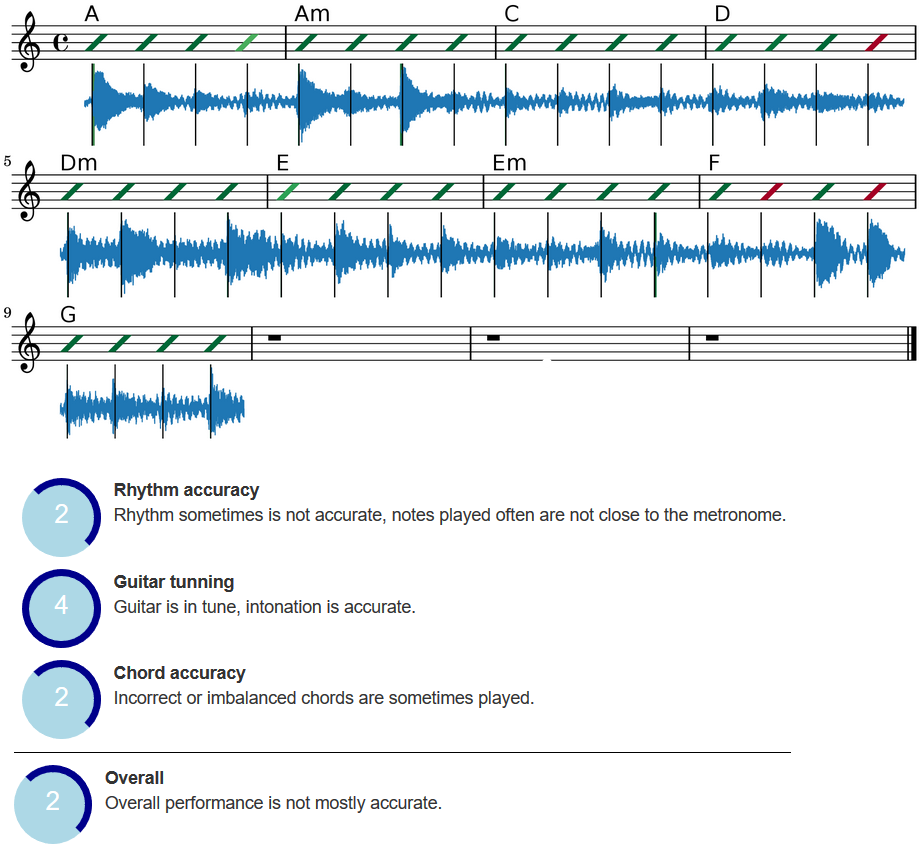
\includegraphics[width=\columnwidth]{introduction/mciritic.png}
    \caption{MusicCritic's feedback interface for a strumming exercise}
    \label{fig:musiccritic}
\end{figure}

\section{Motivation and Objectives}

In automatic assessment systems, the correctness and quality of the played notes and chords are determined by analysing their audio segments and comparing harmonic features with expected results. Accuracy of the assessment in any criteria, particularly rhythm, strictly depends on correct detection of locations of played notes. Therefore onset detection is arguably the most important part of an automatic assessment system.

Guitar players need to move their hands and interact with strings quickly and accurately. Due to its nature of the instrument, unintended noises occur often. Some of these noises (e.g. slide noise) even became a characteristic of guitar and generated by synthesizers to make the audio more realistic. Those noises do not add any musical meaning to the performance. Beginner players, who do not have hand coordination skills yet, generate plenty of noises. For instance, pressing the strings with incorrect posture or weak force usually causes a "buzz" noise, as a result of a loose string collapsing frequently with a fret. Noise events, just like the played notes, change the spectral content in the recorded signal. An onset detection algorithm for a MOOC on guitars must be robust against such noises for the aforementioned reasons. 

In many MIR tasks, most algorithms are developed and tested on high-quality recordings; the players are skilled and recording environments are adequate. Also, there is a post-processing step if it is a commercial recording. Those algorithms show inferior performance on amateur recordings. Most onset detection algorithms in literature also do not address amateur recordings. They are not very useful for applications where users are not highly skilled and the recording environment is non-ideal (e.g. noisy, reverberant), especially if the instrument is a guitar and the player is a beginner. 

Music teachers can distinguish the noises from intended notes easily and assess the performance accordingly. An assessment system to be used in a MOOC for guitars must have a very accurate onset detection algorithm. This is necessary for fair grading, and especially for correct feedback to the students. A grading system, possibly a machine learning algorithm, could tolerate a few detection mistakes. But on a feedback given to the students, obvious mistakes would harm the reputation of the assessment system and the online course.

Objectives of this work are

\begin{itemize}
  \item Evaluate several onset detection algorithms on guitar recordings, including the state of the art algorithm and the one currently being used in MusicCritic.
  \item Develop a better onset detection algorithm by considering the complications of amateur recordings.
  \item Improve the automatic rhythm assessment results using the new onset detection algorithm.
\end{itemize}

We use the rhythm assessment to measure the effect of onset detection algorithms on the overall system since the rhythm assessment depends only on (perceived) onset locations. 

\section{Thesis Organization}

In the next chapter, onset detection methods are reviewed and some studies on perceived attack time are discussed. In chapter 3, the datasets used in this study are described. In chapter 4, annotations of the datasets and evaluations of onset detection and automatic rhythm assessment experiments are explained.

In chapter 5, characteristics of the common noises in guitar recordings are examined. Insights gained from this chapter are used in the development of the new onset detection algorithm, which is explained in chapter 6. Onset detection and automatic rhythm assessment results are presented in chapter 7, followed by discussion and conclusion chapters.

\newpage



\chapter{Related Work}

Studies on automatic musical performance assessment usually adopt the existing algorithms for tasks such as chord detection, automatic transcription or onset detection. A recent overview of performance assessment studies is provided by Lerch et al. \cite{lerch2019mpa}. More general reviews of MIR and music education can be found in \cite{dittmar2012} and \cite{percival2007effective}. 

There are a few studies that develop a new onset detection algorithm, and only one for guitars \cite{eremenko2020performance}. There are no public work focusing on amateur (noisy) recordings or their implications in the context of MOOCs. In this chapter, we review onset detection algorithms in general, focusing on the ones used for guitars or performance assessment systems. 

\section{Onset Detection}

Onset can be defined as the first detectable part of a note event in the recording if the note were isolated \cite{leveau2004}. The task can be separated as offline and online (real-time) onset detection. Some applications provide real-time feedback to the player (e.g. karaoke, Rocksmith\footnote{www.rocksmith.com}, Yousician\footnote{https://yousician.com}) and require online detection. B{\"o}ck et al. \cite{bock2012evaluating} provides an overview for online onset detection. Music performance analysis systems do not necessarily require onset detection in real-time. In MusicCritic, analysis is done after performances are recorded. Therefore we focus on offline onset detection in the rest of the work.

Most existing algorithms can be grouped under signal processing, machine learning or probabilistic methods. There are several reviews \cite{hainsworth2003onset} \cite{collins2005comparison} \cite{bello2005tutorial} \cite{dixon2006onset} available mostly covering signal processing methods. Hidden Markov Models (HMM) are commonly used in several probabilistic methods \cite{abdallah2003unsupervised}, \cite{raphael2010music}.

Signal processing methods rely on spectral energy, phase, pitch, or a combination of those. A musical onset most likely increases the energy of the signal, which simply explains the motivation behind common usage of energy. However in complex situations such as a quiet note is played while another note is decaying, the total energy might not increase. This issue is addressed by discarding the frequencies that are losing energy in spectral flux \cite{spectralflux} (eq. \ref{SF}). Spectral flux is widely used within many other algorithms \cite{holzapfel2009three}, \cite{bock2013maximum}. Wu and Lerch \cite{wu2018learned} combined spectral flux with an adaptive peak picking method for their experiments in assessment of percussive instruments.\\
Spectral energy is often sufficient for detecting the onsets of percussive instruments but not for instruments with slow attacks, such as wind, bowed and voice. As first introduced \cite{bello2003phase}, phase information is found to be useful for non-percussive instruments. The energy of a note with a slow attack may increase steadily for a long duration, which makes it an imprecise indicator of the onset location. Whereas phases of frequencies change abruptly only in the beginning of the attack. However, abrupt changes in phase may arise due to the unreliability of phase processing \cite{holzapfel2009three} or inaudible noises. A common approach is to combine phase information with other onset detection functions. Bello et al. \cite{bello2004use} used both energy and phase information and reported overall improvement over the use of energy or phase only.

Pitch information is especially powerful on monophonic instruments with slow attacks and seldom unwanted noises, such as wind instruments. The absence of noises allows clear detection of pitch over contours. Two recent automatic assessment studies by Vidwans et al. \cite{vidwansobj} and Wu et al. \cite{wu2016towards} take the boundaries of the pitch contours as onsets for wind instruments. For more complex scenarios, pitch information can be combined with energy \cite{tan2010audio} \cite{zhou2007music} or both phase and energy \cite{brossier2004fast} \cite{holzapfel2009three}.

Vibrato and tremolo techniques create fluctuations on pitch and energy of a note. Those fluctuations cause multiple false detections. Vibrato suppression methods are developed on energy \cite{bock2013maximum} and pitch based \cite{collins2005using} detection algorithms to address this issue. 

Özaslan and Arcos \cite{ozaslan2010legato} focused on the identification of playing techniques legato and glissando on classical guitar. Plucked onsets are detected plucked notes with HFC and YIN pitch detection algorithm is used to detect the technique. Laurson et al. \cite{laurson2010simulating} worked on the simulation of the rasgueado technique on the classical guitar, where the notes are very close to each other due to fast strumming. The onsets from the real recording are detected by selecting the peaks of the smoothed total energy of frequencies between 11kHz and 20kHz. 

Mounir et al. \cite{mounir2016guitar} proposed an algorithm for guitar onset detection, which is called NINOS$^2$. After taking the STFT of the audio, the algorithm measures the sparsity of the spectral energy after discarding the frequencies with high energy. The motivation is that the low energy frequencies represent the guitar onsets better, as they usually arise from the interaction of finger (or plectrum) and strings and decay fast. The algorithm predicts the frames as onsets that have low sparsity.

Kehling \cite{kehling2014automatic} developed an automatic transcription system with an onset detection stage. Three existing onset detection algorithms (Spectral flux, Pitchogram Novelty \cite{abesser2017instrument} and Rectified Complex Domain \cite{dixon2006onset}) are applied and combined additively. Each algorithm exploits a different feature; energy, pitch and phase. The combination is found to be performing better than individual algorithms.

In MusicCritic \cite{eremenko2020performance}, Superflux \cite{bock2013maximum} algorithm is used. For the elimination of noises, detections are rejected if the energy difference is less than zero or averaged spectral centroid is more than a threshold. 

Neural network based algorithms, as in many other MIR tasks, perform best in onset detection. According to comparisons in MIREX \cite{mirex} \footnote{https://www.music-ir.org/mirex/wiki/MIREX\_HOME} in the last years, Convolutional Neural Network (CNN) \cite{lecun1998gradient} based algorithms achieve higher detection scores than previous algorithms. The current state-of-the-art onset detection algorithm (CNNOnsetDetector) is also a CNN developed by Schlüter and Böck \cite{schluter2014improved}. Their motivation behind the use of CNN on onset detection is that note onsets create edges in spectrograms and CNNs can learn to detect edges effectively.

\section{Perceived Attack Time}

Physical onset time (PhOT) is the actual acoustic beginning of an audio event, perceptual onset time (POT) is the moment listeners perceive the event and perceptual attack time (PAT) is defined as the perceived moment of rhythmic placement of the event \cite{wright2008shape}. Most onset detection studies aim to find PhOT or POT of musical events. Although physical onset is useful for analysis of the audio, PAT is more accurate for rhythmic performance assessment. Polfreman \cite{polfreman2013} evaluated nine different onset detection algorithms on five different onset types, concluding that the algorithms are not suitable to detect PAT of non-percussive sounds. 

On guitars, POTs of single notes are close to their PATs, since the instrument is plucked and percussive. This is not the case for strummed chords. A strummed chord is a single musical object that consists of multiple onsets close to each other. Hove et al. \cite{hove2007sensorimotor} showed that the PAT (they used the term perceptual center) of two close tones depends on the pitch of the tones, their order, and the amount of time between them. 
    
Frerie et al. \cite{freire2018strumming} studied the beat location of guitar strums perceived by the players. In their experiment, the same excerpts are played by different musicians on an acoustic guitar with hexaphonic pickups to record each string. Results showed that each player aligns chords to the metronome differently.

\chapter{Datasets}

This section describes the datasets used in this work. Onset detection algorithms are evaluated on two datasets; GuitarSet and MusicCritic dataset. They represent two different ends and complement each other. In MusicCritic dataset, simple exercises are played in environments that are not high quality and diverse. In GuitarSet, performances are complex and fast, recorded in a soundproof studio. For automatic rhythm assessment, we use MusicCritic dataset.

\section{GuitarSet}

This dataset \cite{xi2018guitarset} contains 360 recordings total of 183 minutes. Half of them are solo (mostly single notes) and the other half is the corresponding accompaniment (chords) tracks. Six players with more than 10 years of experience are given lead sheets and asked to play accompaniment and then solo over their accompaniment. Performances include various keys, tempi, and genres. Each string is recorded and annotated separately using a hexaphonic pickup. Onsets are automatically generated and then manually corrected. Dead notes that are not audible and non-note events are discarded from the onset annotations.\\ 
In this work, we use mono microphone recordings for the onset detection task. Onset locations of each string are taken from the annotations and onsets that are close to each other (e.g. strummed chords) are merged.


\section{MusicCritic Dataset}

This dataset \cite{eremenko2020performance} contains 232 recordings. 107 of them contain only chords and the rest of them only single notes. Six exercises (3 chord and 3 single note) are performed by players with various skill levels. Recordings are made with different setups and guitars. Two guitar teachers graded the recordings, from 1 to 4, on rhythm accuracy, pitch accuracy, guitar tuning, and overall performance. Onsets are manually annotated as explained in section \ref{mc_annot}.

\section{Guitar Noises Dataset}

Examination of guitar noises would contribute to both onset and noise detection and synthesis of realistic guitar sounds. But there are no public datasets for such noises. We created a dataset that contains buzz and slide noises from wound strings of a classical guitar. Our aim is to understand the nature of these noises better and develop the onset detection algorithm accordingly. See appendix \ref{appendix:b} for details. \\

\chapter{Methods}

In this chapter, onset annotation, onset detection evaluation, automatic rhythm assessment and its evaluation are explained. 

\section{Onset Annotations of Datasets}

\subsection{MusicCritic Dataset}\label{mc_annot}
Recordings are manually annotated by the author, using the Sound Annotation & Analysis Tool (see Appendix A for details) developed during the course of this work. This tool made the analysis of the sounds and comparison of algorithms easier. It can display many audio features from Essentia \cite{essentia} library and predictions of multiple onset detection algorithms on its interactive plots.

Prior to the annotation session, two buttons are assigned to stamps "Onset" and "Crop". "Onset" stamp is used for onsets of single notes and chords. "Crop" is used at the beginning and end of the recordings to remove silenced or unrelated parts. Annotation is done by pressing the stamp on the keyboard and clicking on the plot. The annotator can start and stop playing recordings freely during the process. A moving cursor is aligned with the sound being played to show the location. The annotator wore headphones in a quiet environment. Both visual and aural cues are used in determining the onset locations.  

For a single note, the maximum location of the waveform is selected as the onset time. For a chord, the first perceivable note is aimed on the waveform. On each recording, the plot is zoomed to contain at most 4 onsets. When the visual cue is weak (e.g. a weak note is played when the previous note is not decayed yet), annotation is done after additional zoom and repeated listening.

\subsection{GuitarSet}
Onset annotations of GuitarSet are already available, but they are separate for each string. We deduce the onset locations of strings in a chord to a single location. Onset locations that are closer than 0.025 ms are grouped (e.g. 6 string chord may span up to 0.125 ms) and then their average is taken as the chord onset. Apart from taking the average, last onsets and first onsets are also tested in evaluations. The effect on overall scores is found to be negligible.

\section{Evaluation of Onset Detection Algorithms}

The mir\_eval \cite{raffel2014mir_eval} library is used for onset detection evaluation. The evaluation method is the same as the method used in MIREX evaluations. An onset is correctly detected if there is an onset prediction inside the tolerance window. The standard size of the tolerance window is 50 ms. If there are more than one prediction for the same true onset (called the doubled onsets), excess predictions are added to the false positive onsets. If there is one prediction for two onsets (called the merged onsets), excess true onsets are added to the false negative onsets.

TP: True Positive
FP: False Positive
TN: True Negative
FN: False Negative

Precision \(P = \frac{TP}{TP+FP}\)\\
Recall \(R = \frac{TP}{TP+FN}\)\\
F-score \(F = \frac{2\cdot P\cdot R}{P+R}\)\\

A set of onset detection algorithms (Complex \cite{bello2004use}, Complex Phase \cite{brossier2004fast}, Superflux \cite{bock2013maximum}, NINOS$^2$ \cite{mounir2016guitar},  HFC \cite{masri1996imroved}, RNNOnsetDetector \cite{eyben2010universal}, CNNOnsetDetector \cite{schluter2014improved}) are evaluated on GuitarSet with the standard tolerance window size of 50 ms (Table \ref{tab:GSothers}). The most promising algorithm (CNNOnsetDetector), together with MC-OnsetDetector and the algorithm developed in this work are evaluated on both GuitarSet and MusicCritic datasets. This time the evaluation is more detailed.

Nearly half of each dataset consist of chords. Chords' attack time may vary depending on the strumming speed of the player, and it may exceed the tolerance window size. There is no consensus on the onset location of a chord and algorithms may aim at different locations on the sound envelope. To make the evaluation fair, onset predictions are re-evaluated eleven times by shifting them, from -50 ms to +50 with 10 ms increments. The highest F-score among those evaluations is accepted as the score of the algorithm. 

\section{Automatic Rhythm Assessment}\label{assessmethod}

The automatic rhythm assessment algorithm consists of three parts: onset detection, processing (feature extraction), and prediction. In the processing part, features are created using the predicted onsets. Those features are then used to predict the grades. We keep the processing and prediction parts the same with the previous work  \cite{eremenko2020performance} and the evaluation as well, to measure the effect of different onset detection algorithms. The problem is that it is not clear how to process the onset locations for rhythm assessment. There are a few studies where onset locations are processed for rhythm assessment \cite{percival2008thesis} \cite{abesser2014automatic} \cite{wu2016towards} \cite{falcaoMast}, but they are evaluated on different datasets. Here we explain how the onsets are processed in this work. Our aim is to identify a minimal processing method that allows a fair comparison of the onset detection algorithms.

In the previous work, predictions were made by applying isotonic regression \cite{mair2009isotone} to processed onsets. In this work, we do the same. In the processing part, deviations of onset predictions from the metrical positions were taken. The metrical positions are aligned with a metronome that students can hear while playing. This method is not accurate when the chords are strummed. On strummed chords, beat location is not clearly defined. Players choose the beat location subjectively \cite{freire2018strumming}. Beat location is subjective also for the listeners \cite{hove2007sensorimotor}. This means that the difference between an onset prediction and the metronome beat is not enough to determine the timing of the chord. For this reason, a different method is used in this work. We argue that the time differences between onset predictions are better features than the differences between onsets predictions and metronome beats. For the following reasons: 

\begin{itemize}
  \item In a recording, the factors that affect the characteristics of a strummed chord (e.g. player, instrument, recording device and the environment) stays the same. It can be assumed that the characteristics of the strummed chords (or the single notes) in that recording are with each other, when compared to chords from different recordings.
  
  \item In a recording where the characteristics of strummed chords are consistent, it can be assumed that the locations of onset predictions of an algorithm are also going to be consistent.  
\end{itemize}

Perceived beat locations are also consistent for players \cite{freire2018strumming} and listeners \cite{hove2007sensorimotor}. If all of the consistencies in the assumptions were perfect, the time differences of onset predictions would be equal to the time differences of the listener's (and player's) beat locations (e.g. in Figure \ref{fig:devi}, differences between red lines are equal to the differences between green lines). If the consistencies are not perfect, the time differences are not equal but still correlated. So, the time difference of onset predictions represents the perceived beats better than the differences from the metronome beats, since the differences from the metronome beats are subjective. 

We normalize the time differences by their tempo, so the machine learning algorithm can be used effectively. Normally, we should take the deviations of time differences from the corresponding beat duration. Since the exercises in the MusicCritic dataset only contains quarter notes, we can use the deviations from the tempo directly. 

\begin{figure}
    \centering
    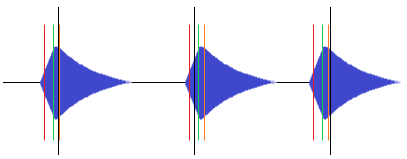
\includegraphics[width=\columnwidth]{methods/devi.png}
    \caption{A toy example of identical strummed chords. Timing of a strummed chord can only be understood when it is compared to other chords. Given three chords, the chord in the middle is played late. (Black line is metronome. Red, green and orange lines are onset predictions, listener's beat locations and student's beat locations, in any order.)}
    \label{fig:devi}
\end{figure}

In the prediction part, the isotonic regression is applied to onset difference deviations to predict the rhythm grades of the MusicCritic dataset.


\chapter{Common Noises in Guitar Recordings}

Noises can be separated into two categories, instrument and environment noises. We expect instrument and environment noises because in our use case, an online musical instrument course, we do not expect players to be experts, or to have access to an isolated recording environment. Our aim is to make an automatic assessment system robust to such noises. 

Most common instrument noises in amateur guitar recordings are \textit{slide} and \textit{buzz} noises. Slide noises are more common as they can be heard on all levels of performances. So common that they are artificially generated by guitar synthesizers to make the sound more realistic \cite{pakarinen2007analysis}. Buzz noises however, do occur most when the player is a beginner. Buzzing sound is considered unpleasant and unwanted. Another common noise is the percussive sound generated when right hand (or picking hand) touches excited strings. The touch could be intended to mute the string. The noise could also be intended, to add rhythmic percussion to the performance. In any case, it is classified as noise in this study. Environment noises are not predictable as instrument noises. There are too many possibilities for unwanted sounds in a non-ideal recording environment. One specific environment noise which might be expected in our use case is computer fan noise.

\section{Slide Noises}

Slide noises mostly happen during chord transitions. They occur when players move their hands while touching the strings. On nylon strings, they are much less audible. We focus on wound strings when we talk about slide noises. 

Pakarinen et al. \cite{pakarinen2007analysis} provides an analysis for these noise sounds. Sound consists two components. First, time-varying harmonics generated from interaction of finger and winding turns and second, static harmonics due to longitudinal vibration of the string. Energy of the time-varying harmonics are higher than static harmonics. 
\begin{equation}\label{slide_eq}
    f_H_n = nv_sd_w \quad, \quad n \in \mathbb{Z}^+
\end{equation}
Frequencies of the time-varying harmonics are linearly proportional to the speed of the finger (\(v_s\)) and wound density (\(d_w\)). As finger passes through each single winding turn, an impulse is created. Faster movement or denser winding turns result in shorter period between impulses. Static harmonics are due to vibration of the string, so they are not affected by the speed of the finger. Vibrations are only on longitudinal axis, since transversal vibrations are damped by the finger. Frequencies of the harmonics of longitudinal vibrations depend only on the length of the string and the density of its material. Therefore frequencies do not change with respect to location of sliding, but only their magnitudes.   
  
If the player tries to move his hand while still pressing on a string, the sliding noise will have higher initial energy and its pitch will be perceivable. In this form, the noise is often referred as a 'squeak' noise. The difference is the speed of the finger. Due to static friction between the string and the finger tip, the finger tip does not move immediately. While the player reduces the pressing force on the strings, at one moment, the force of static friction falls below the force acting on fingers parallel to the fret board, which was holding the whole arm from moving. Thus the instantaneous velocity of the finger at the moment it starts moving is much more higher than what it should be with a proper playing technique, causing an unpleasant 'squeak' sound. \\

Acceleration and deceleration of the hand between two frets causes frequencies of the time-varying harmonics to increase and then decrease (Figure \ref{fig:slide}). This trend was also found in \cite{pakarinen2007analysis}. 


\begin{figure}
    \centering
    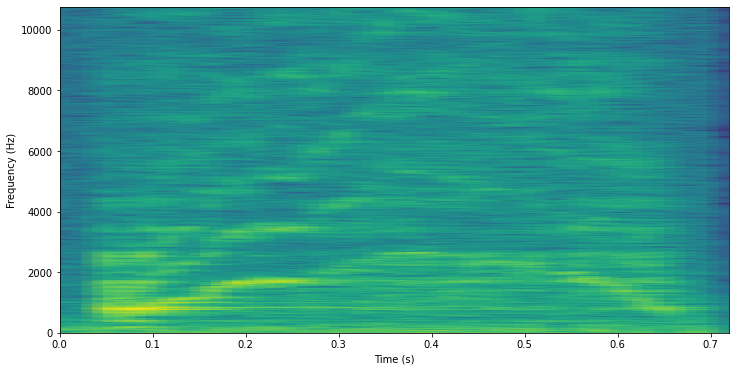
\includegraphics[width=\columnwidth]{methods/S_NR_A_12to3_stft.png}
    \caption{Short-time Fourier Transform magnitudes of the slide noise generated between 12th fret and 3rd fret of A string}
    \label{fig:slide}
\end{figure}

\section{Buzz Noises}\label{buzzsection}

These noises occur when a string collides with a fret during vibration. Collision of string and fret generates high frequency components. If the player does not apply enough pressing force between two frets, plucked string periodically leaves and collides with the fret of the note the player trying to play. Buzz noises also occur due to construction errors (e.g. unequal fret heights) or poor adjustments on the guitar (e.g. incorrect neck relief, height of the bridge and the nut).

Buzzing is a characteristic behaviour of Indian instrument sitar, and is not classified as a noise. Realistic synthesis of sitar sound requires modelling of the collision of strings and the bridge of the sitar. Vyasarayani et al. \cite{vyasarayani2009} models the movement of string in three phases. In first phase, plucked string do not contact with the obstacle (bridge). In second phase, the string partially wraps the obstacle. Lastly, the obstacle is completely wrapped. This description of string movement can be adapted to modelling of buzzing noise in the guitar. In case of guitar, obstacle is fret instead of bridge. One important difference is that the obstacle on guitar (fret) is circular and is never completely wrapped by the string. Third phase in movement of sitar string does not exist in guitar.     
  
Length of the string in motion is different in two phases (Figure \ref{fig:buzz}) . Length in first phase is greater than in second phase, by distance between the finger and the fret. If the buzzing is caused by weak force on the pressing finger (instead of an error on the guitar) we expect the frequency of produced sound to be lower due to the change of length. We see one example from our noise dataset on Figure \ref{fig:buzzstft}, where note B2 is played on E string (standard tuning). Buzz noise is generated by slowly releasing the string, which begins around 0.12 seconds. Fundamental frequency (F0) (Figure \ref{fig:buzzf0}) is obtained using YIN \cite{de2002yin} algorithm. F0 decreases from ~123 Hz (B2) towards ~116 Hz (A#2), but does not reach to it. Frequency of the decreased F0 depends on location of the finger on the fret.


\begin{figure}
    \centering
    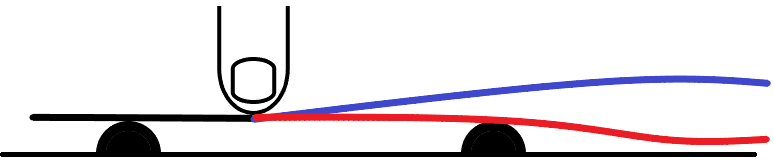
\includegraphics[width=\columnwidth]{methods/buzz_mov2.png}
    \caption{Phases of string motion during a buzz noise. Bottom line and half circles represent fretboard and frets. (Blue: Phase 1, Red: Phase 2)}
    \label{fig:buzz}
\end{figure}

\begin{figure}
    \centering
    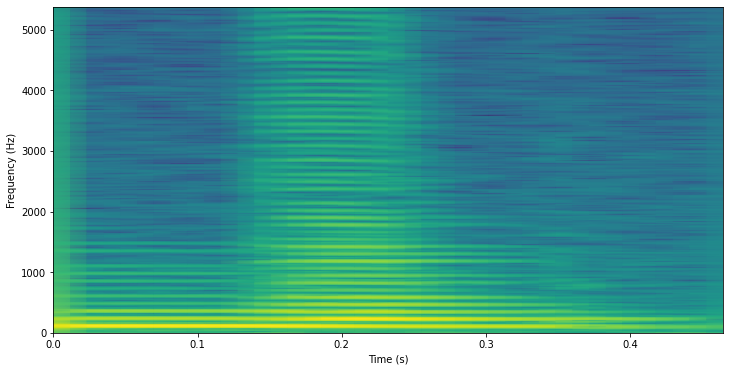
\includegraphics[width=\columnwidth]{methods/B_E_7_stft.png}
    \caption{Short-time Fourier Transform magnitudes of the buzz noise generated on 7th fret of E string}
    \label{fig:buzzstft}
\end{figure}

\begin{figure}
    \centering
    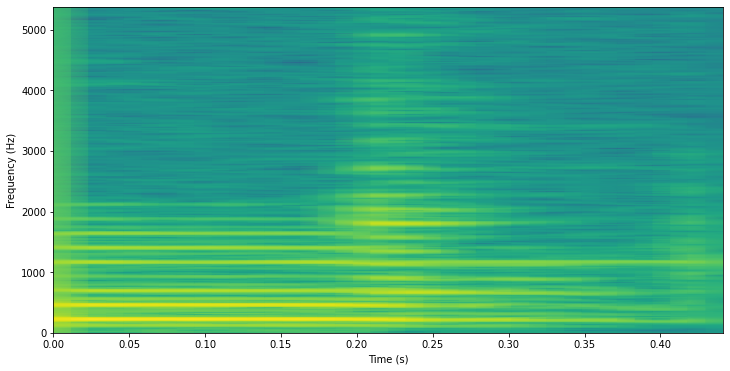
\includegraphics[width=\columnwidth]{methods/realbuzzstft.png}
    \caption{Short-time Fourier Transform magnitudes of the buzz noise in a recording from Music Critic dataset}
    \label{fig:realbuzz}
\end{figure}

\begin{figure}
    \centering
    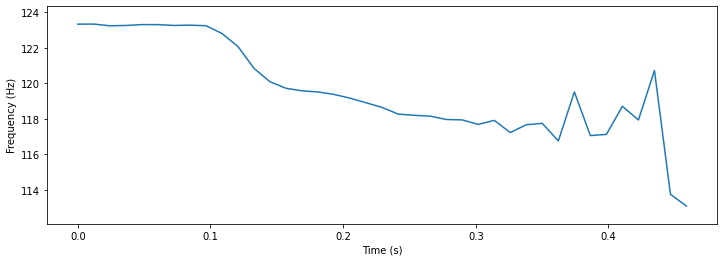
\includegraphics[width=\columnwidth]{methods/B_E_7_f0.png}
    \caption{Fundamental frequency of the buzz noise generated on 7th fret of E string}
    \label{fig:buzzf0}
\end{figure}

Buzz and slide noises cover most of the unintended noises in guitar recordings. There are also unpredictable noises that do not arise from fretboard and players hands, such as background noises or random sound producing events in the recording environment. Players may not have the complete control of their recording environment to prevent such noises. An onset detection algorithm must be robust to distinguish noises from players performance, just like a music teacher could do.
\chapter{Harmonic Onset Detector Algorithm}

An ideal onset detection algorithm would detect all the played notes and eliminate all noises. The algorithm can be built on the differences between the noises and musical notes.   

All events, noises and notes, introduce changes to the energy distribution of the frequencies. Some events, may not cause an increase of the total energy. For example, during a glissando, the played note changes without an energy increase. Therefore, frequency domain representation of the audio signal is suitable for detecting guitar (and many other pitched instruments) note onsets. Crucial step is to find the differences of noises and notes in that representation.

Most useful property of guitar notes is that they are harmonic. This property can be exploited to separate notes from various inharmonic noises. For slide and buzz noises, which are harmonic, further inspection is needed. Unstability of the frequencies of the slide noises can be used to eliminate slide noises. Fundamental frequency (f0) of the sound event can also be used for determining a note, fundamental frequency of a slide noise is usually greater than f0 of possible guitar notes. For example, average of the hand speed in the slide noise shown in Figure \ref{fig:slide} is approximately 0.45 m/s (distance between frets divided by slide duration) and average fundamental frequency is 1800 Hz (using the equation \ref{slide_eq}, \(d_w \approx 4000 \) windings per meter). A slide noise with faster hand speed can surpass the highest possible fundamental frequency on a guitar with standard tuning, which is 1975 Hz (B6). In the case of buzz noises, frequencies of the harmonics are stable. Most distinguishable property of buzz noises is their duration are quite short compared to notes. Figure \ref{fig:buzz} shows a buzz noise that lasts around 0.1 seconds. That buzz is generated intentionally and is quite longer than buzz noises found in performance. In Figure \ref{fig:realbuzz} we see a naturally occurring buzz noise in a beginners performance. Given the properties of notes and noises, an onset detection algorithm can be built according to following argument: \\ At a given time point, a guitar note onset exists if there is at least one harmonic series in the differences of energy magnitudes of frequencies after and before the time point, and that harmonic series lasts longer than minimum expected note duration. There are more than one ways to create an algorithm to detect guitar notes in the way they are described in the argument above. In the remaining of this section, design and parameter choices of the developed algorithm is discussed.

Detecting and tracking the harmonic series requires a time-frequency representation of the audio signals. Short-time Fourier Transform is the first step of the algorithm. Detecting harmonic series on a time frame requires calculations over peaks of the spectrum, which will be called the \textit{harmonic analysis} step. Duration of a harmonic series is calculated by tracking the harmonic series through successive time frames, which is called the \textit{segmentation} step. Those two steps (harmonic analysis and segmentation) brings computational expense. Applying them on every time frame is not practically possible. Therefore an \textit{onset candidate selection} step is required before those steps. The candidate selection step should be much cheaper, as it is applied to all time frames. Details of each step is described in following sections. The overall algorithm consisting those steps is referred as Harmonic Onset Detector.

\begin{figure}
    \centering
    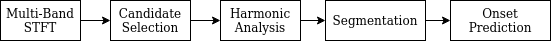
\includegraphics[width=\columnwidth]{methods/overall.png}
    \caption{Overall scheme of Harmonic Onset Detector algorithm.}
    \label{fig:scheme}
\end{figure}

\section{Short-Time Fourier Transform}
Separating lower frequencies require a larger window size, but a large window size causes smoothing in time, decreasing the time accuracy of the onset detection algorithm. Using different window sizes for different frequency bands solves this problem at the expense of computation. The following parameters are found to be working well in experiments.

Bands (Hz): (0-1000), (1000-5000), (5000 - \(F_s / 2\)) \\
Window Sizes: 8191, 2047, 1023\\
Window: Blackman
FFT Size = 8192\\
Hop Size = 128 

Where  \(F_s\) is the sampling rate. The window size of the lowest band is not large enough to separate the two closest frequencies on a guitar with standard tuning (82.41 Hz and 87.31 Hz). This does not prevent the detection of low frequency notes because the detection of the harmonic series is done with an error tolerance. Even if the fundamental frequency (f0) is not separated, higher harmonics (f1,f2...) are separated and the existence of a new harmonic series can be detected from those higher harmonics.

\section{Candidate Selection}

This step is required to avoid applying the rest of the algorithm on all time frames. Spectral flux \cite{spectralflux} is the sum of the positive differences of frequency magnitudes. It measures the positive change between consecutive time frames. Originally, the summation includes all frequency bins. Experiments showed that limiting the frequency bins between possible fundamental frequencies of guitar improves the performance of candidate selection. Bins are limited between two bins below the minimum frequency (82 Hz) and two bins above the maximum frequency (1975 Hz). Bins corresponding to these frequencies can be calculated using FFT size.

\begin{equation}\label{SF}
    SF(t) = \sum_{k=N_{82Hz}-2}^{N_{1975Hz}+2} H(|X(t,k)|-|X(t-1,k)|)
\end{equation}

Where $H$ is the half wave rectifier and $t$ denotes the time frame. SF is normalized between 0 and 1, \( SF = SF / \max |SF|\)  and then smoothed by using a Savitzky-Golay filter \cite{savgol} with window size (\(w_{SG}\)) of 51 and polynomial order of 3. The size of the window can be converted to time by multiplying with (Hop Size \(/ f_s\)), which is 0.148 ms in this case. The main contribution of this smoothing step is to reduce the number of candidates in strummed chords.

A simple peak picking algorithm is used on smoothed SF to select candidates. A time frame is selected as an onset candidate if SF(t) is maximum between the time window \((t-\lfloor w_{SG}/2\rfloor, t+\lfloor w_{SG}/2\rfloor) \) and is greater than the average inside that window by a small threshold of 0.01.  

\section{Harmonic Analysis}

STFT magnitudes after and before the onset candidate are compared to determine the existence of new harmonic series. 160 frames around onset candidates (80 left, 80 right) are used for the analysis. The analysis window shortens if there is another onset candidate closer than 80 frames (if not, an inharmonic noise just before a true onset would be falsely predicted as an onset).  Keeping the number of frames for analysis on the right side of the onset candidate is important for the accuracy of the algorithm. Onset candidates are therefore analysed starting from the latest and removed from the candidate list if they are not predicted as onsets, allowing the previous (in time) onset candidate to be analysed on 80 frames on the right side.

Two windows of frames just before and after the candidate are used to determine the frequencies that gained energy. The lengths of those windows are equal to half of the total number of analysis frames on each side. Windows are moved away from the onset candidate so they contain less smeared energy and frequencies with increased magnitude can be more accurately detected. The average magnitude of each frequency bin is calculated inside two windows and compared. Frequency bins that have not gained energy above a threshold are masked. So the algorithm only seeks for harmonic series inside the frequencies that gained energy. This way, an inharmonic noise will not be falsely predicted as an onset when there is already some harmonic content.

For each time frame, peaks on the spectrum are detected and another frequency masking is applied. Peaks are eliminated if they are close to a peak with much higher energy. The aim is to eliminate the perceptually masked frequencies and to reduce the computation of the harmonic series search. This perceptually motivated masking is not a realistic simulation of human perception, it is meant to be quite simple and computationally cheap. Figure \ref{fig:crude_mask} shows an example of the masking. 

From the remaining peak locations, the first 10 peaks in the range of the guitar are selected as f0 candidates. Possible missing f0 candidates are generated by dividing higher peak frequencies by 2 and 3, then added to the f0 candidate pool. Error for each harmonic series is calculated as follows:\\
$H$: Highest harmonic considered in the error calculation \\
\(D(nf0)\): distance of $n^{th}$ harmonic to the closest frequency peak \\
\(r(nf0)\): error of the $n^{th}$ harmonic \\
\(R(F0)\): total weighted error of the harmonic series

\begin{equation}\label{nerror}
    r(nf0)= \begin{cases} 
          D(nf0) & D(nf0)\leq 2n \\
          30 & D(nf0) > 2n 
          \end{cases}
\end{equation}  

If $D(nf0)$ is greater than $2n$, $n^{th}$ harmonic is marked as non-existent. After the error calculation of all harmonics (from 1 to H), error values are weighted using the equation (\ref{wnerror}), where $p$ is the number of harmonics that are found to be existent and $c$ is strictness constant. The total error of the harmonic series is the summation of weighted errors (\ref{toterror}). \

\begin{equation}\label{wnerror}
    r(nf0) =  r(nf0)\cdot e^{-n / e^{H-p+c}}
\end{equation}  
\begin{equation}\label{toterror}
    R(F0) =  \sum_{n=1}^{H} r(nf0)
\end{equation}

\begin{figure}
    \centering
    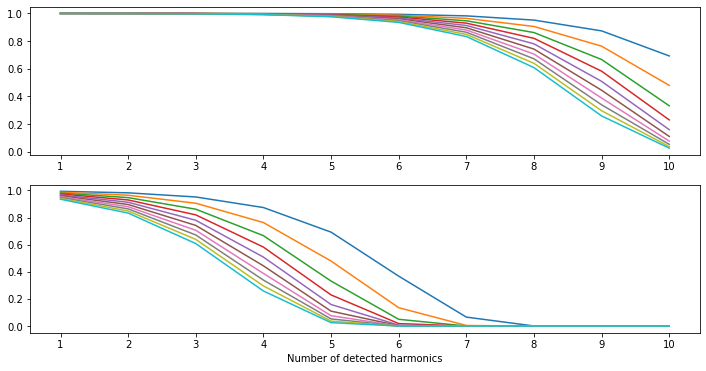
\includegraphics[width=\columnwidth]{methods/hweights.png}
    \caption{Weights of harmonic errors (top to bottom, $0^{th}$ to $(H-1)^{th}$ harmonic) w.r.t. number of existent harmonics. $H = 10$, $c = 0$ (above) and $c = -5$ (below). }
    \label{fig:hweights}
\end{figure}

Equation (\ref{fig:hweights}) adds two things to algorithm. First, the existence of a frequency peak close to a harmonic value is acknowledged directly, the total error decreases with the number of detected harmonics. Second, lower harmonics have more importance. The strictness constant ($c$) is chosen to be -1 in this algorithm. Figure \ref{fig:hweights} shows how $c$ affects the weights.

\section{Segmentation}

Detected harmonic series are tracked through successive frames. The existence of the harmonic series is decided by an error threshold, $t_{he}$. If a harmonic series exists in $n$ consecutive frames, it forms a segment of length $n$. In a segment, harmonic series are allowed to deviate from previous ones to neighboring series, making the segmentation robust against small frequency deviations. The total duration of a harmonic series is calculated by summing the length of its segments. Error and length thresholds are defined and explained below.

Harmonic series error threshold ($t_{he}$) = 200 \\
If the error of a harmonic series in a frame is below  $t_{he}$, it starts or continues the segment at the current frame. If it is above and there is a segment up to this frame, the segment ends. 

Segment error threshold ($t_{se}$) = 80 \\
If the average error of a harmonic series along a segment is greater than $t_{se}$, the segment is eliminated. $t_{he}$ is greater than $t_{se}$, which means higher errors are tolerated for single frames so the segments are not disrupted, but average error along the segments must be lower. 

A numerical example: if 3 harmonics of a series are missing for every frame on a segment and the remaining 7 harmonics are found without any distance error, the total unweighted error would be 90, surpassing the threshold. If the missing harmonics are $7^{th}$,$8^{th}$ and $9^{th}$, which have lower weights than the lower harmonics, total weighted error would be 76.3. In that case, the segment is not eliminated and its length is added to the total length.    \\\\
Segment length threshold ($t_l$) = 8 frames \\
If the length of a segment is less than $t_l$, the segment is eliminated. \\\\
Total length threshold ($t_L$) = 30 frames\\
If the total length of segments of a harmonic series is less than $t_L$, the harmonic series is not accepted as evidence of a guitar note. If it is greater or equal, the onset candidate is predicted as a note onset. 

If there is at least one harmonic series that satisfy the condition above (total length of the segments $\geq t_L$), the onset candidate is predicted as a guitar onset.

A guitar note and a buzz noise are shown in Figures \ref{fig:gs_0_note} and \ref{fig:gs_0_noise}. Both candidates are predicted correctly.

\begin{figure}
    \centering
    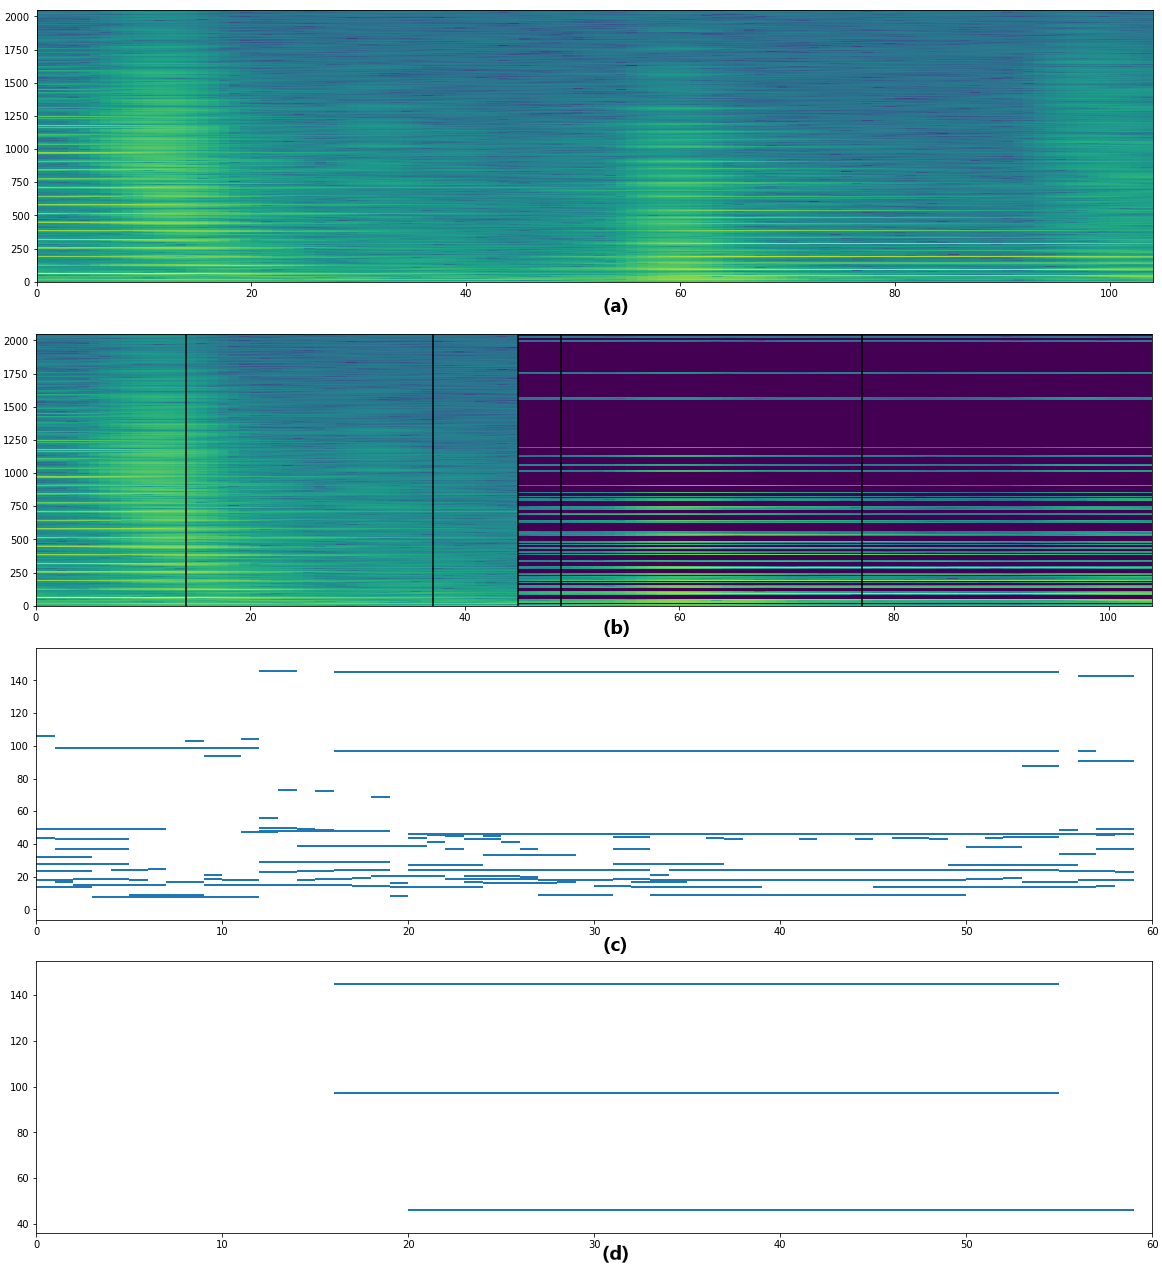
\includegraphics[width=\columnwidth]{methods/gs_0_788_note.png}
    \caption{Visualization of an onset candidate being processed (x: time frames, y: frequency bins). (a) STFT around the onset candidate, (b) Elimination of frequencies after the candidate. Middle line: onset candidate, two lines on both sides: boundaries for frequency elimination calculation. (c) Segments of harmonic series before error and duration thresholds are applied (the candidate is at time frame 0), (d) Remaining segments that are accepted as evidences of a note onset }
    \label{fig:gs_0_note}
\end{figure}

\begin{figure}
    \centering
    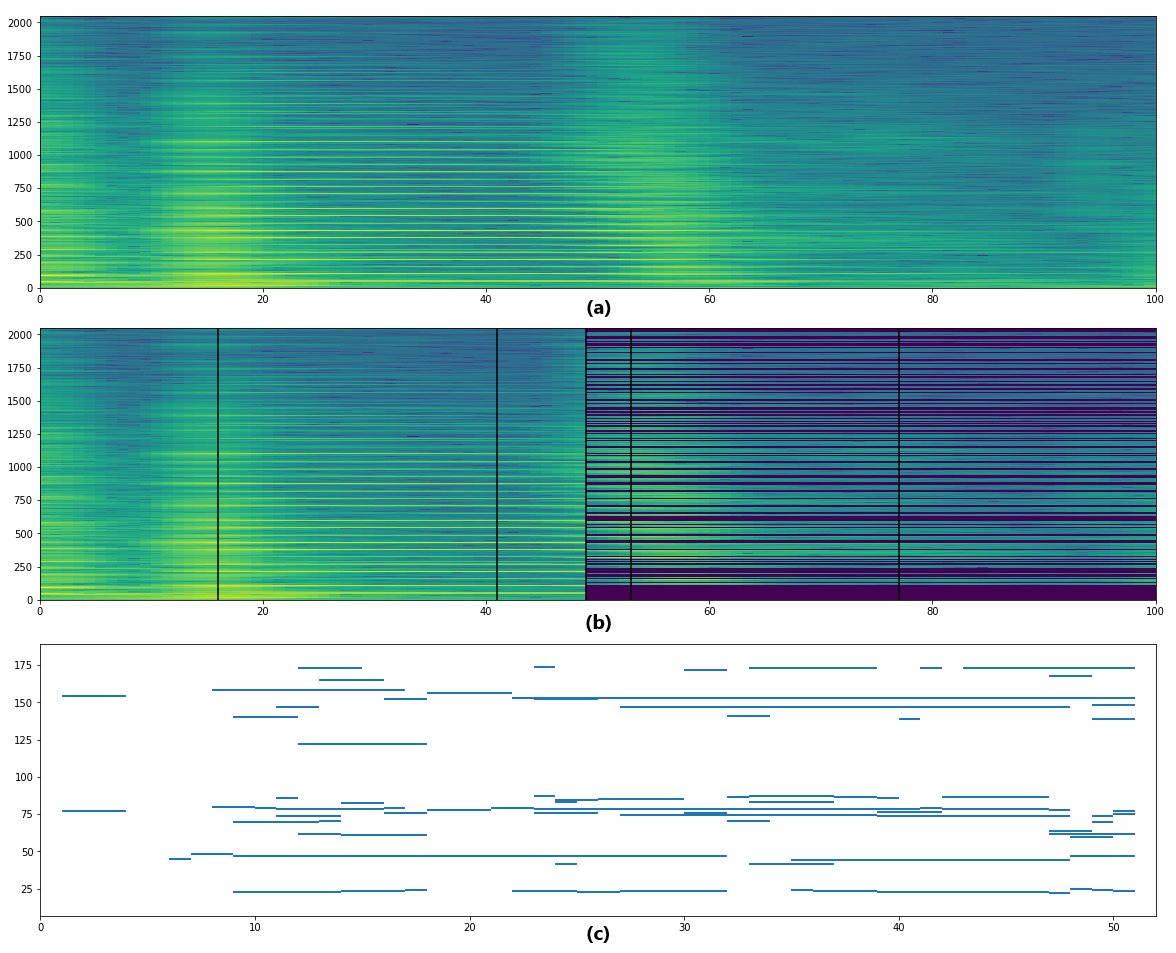
\includegraphics[width=\columnwidth]{methods/gs_0_642_noise.png}
    \caption{Visualization of an onset candidate being processed (x: time frames, y: frequency bins). (a) STFT around the onset candidate, (b) Elimination of frequencies after the candidate. Middle line: onset candidate, two lines on both sides: boundaries for frequency elimination calculation. (c) Segments of harmonic series before error and duration thresholds are applied (the candidate is at time frame 0). All segments are eliminated after thresholds are applied.}
    \label{fig:gs_0_noise}
\end{figure}

\begin{figure}
    \centering
    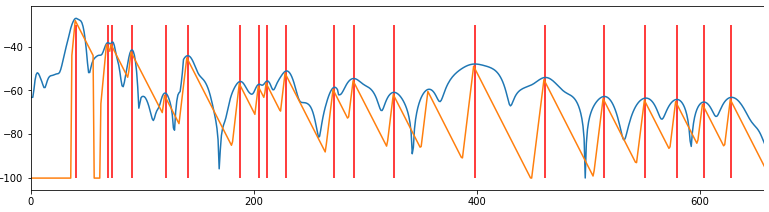
\includegraphics[width=\columnwidth]{methods/crude_masking_r.png}
    \caption{Elimination of frequency peaks in a single time frame. A triangle mask (orange) is created around each peak (red). Peaks that remain under mask are eliminated, such as the peak at 100 Hz.}
    \label{fig:crude_mask}
\end{figure}

\chapter{Results}

Evaluation results of onset detection algorithms and automatic rhythm assessments are presented in this chapter. In the first experiment, various onset detection algorithms are evaluated on GuitarSet. CNNOnsetDetector is found to be performing best among them (Table \ref{tab:GSothers}). Three onset detection algorithms (CNNOnsetDetector, MC-OnsetDetector, Harmonic Onset Detector) are evaluated on both GuitarSet and MusicCritic dataset as explained in methods section (Tables \ref{tab:threeGS} and \ref{tab:threeMC}). Effects of tolerance window size are shown in Figures \ref{fig:wsize_gs} and \ref{fig:wsize_mc}.
\begin{table}
 \begin{center}
 \begin{tabular}{|l|l|l|l|}
  \hline
     & F-score & Precision & Recall \\
  \hline
  Complex & 0.67  & 0.87 & 0.59 \\
  Complex Phase & 0.59 & 0.78 & 0.52  \\
  Superflux & 0.59 & 0.46 & 0.92  \\
  NINOS$^2$ & 0.37 & 0.47 & 0.52  \\
  HFC & 0.65 & 0.79 & 0.60  \\
  RNNOnsetDetector & 0.68 & 0.82 & 0.65 \\
  CNNOnsetDetector & 0.83 & 0.78 & 0.90 \\
  \hline
 \end{tabular}
\end{center}
 \caption{F-score, Precision and Recall of various onset detection algorithms on GuitarSet}
 \label{tab:GSothers}
\end{table}

\begin{table}
 \begin{center}
 \begin{tabular}{|l|l|l|l|}
  \hline
  \textbf{Overall} & F-score & Precision & Recall \\
  \hline
  MC-OnsetDetector & 0.80 & 0.80 & 0.80 \\
  CNNOnsetDetector & 0.70 & 0.59 & 0.92 \\
  Harmonic Onset Detector & 0.85 & 0.86 & 0.84 \\
  \hline
  \hline
  \textbf{Chords} &&& \\
  \hline
  MC-OnsetDetector & 0.74 & 0.74 & 0.74 \\
  CNNOnsetDetector & 0.59 & 0.46 & 0.93 \\
  Harmonic Onset Detector & 0.84 & 0.84 & 0.85 \\
  \hline
  \hline
  \textbf{Single notes} &&& \\
  \hline
  MC-OnsetDetector & 0.85 & 0.86 & 0.84 \\
  CNNOnsetDetector & 0.78 & 0.69 & 0.92 \\
  Harmonic Onset Detector & 0.85 & 0.88 & 0.84 \\
  \hline
 \end{tabular}
\end{center}
 \caption{Performances of three onset detection algorithms on MusicCritic dataset}
 \label{tab:threeMC}
\end{table} 

\begin{table}
 \begin{center}
 \begin{tabular}{|l|l|l|l|}
  \hline
   \textbf{Overall} & F-score & Precision & Recall \\
  \hline
  MC-OnsetDetector & 0.71 & 0.95 & 0.59 \\
  CNNOnsetDetector & 0.84 & 0.78 & 0.92 \\
  Harmonic Onset Detector & 0.84 & 0.89 & 0.81 \\
  \hline
  \hline
  \textbf{Chords} &&& \\
  \hline
  MC-OnsetDetector & 0.69 & 0.95 & 0.56 \\
  CNNOnsetDetector & 0.82 & 0.78 & 0.88 \\
  Harmonic Onset Detector & 0.81 & 0.91 & 0.76 \\
  \hline
  \hline
  \textbf{Single notes} &&& \\
  \hline
  MC-OnsetDetector & 0.73 & 0.95 & 0.60 \\
  CNNOnsetDetector & 0.86 & 0.79 & 0.95 \\
  Harmonic Onset Detector & 0.86 & 0.88 & 0.86 \\
  \hline
 \end{tabular}
\end{center}
 \caption{Performances of three onset detection algorithms on GuitarSet}
 \label{tab:threeGS}
\end{table} 

On average, Harmonic Onset Detector has the highest F-score among three algorithms (Table \ref{tab:threeMC} and \ref{tab:threeGS}). On GuitarSet (Table \ref{tab:threeGS}), CNNOnsetDetector and Harmonic Onset Detector have close F-scores in both chord and single note recordings. MC-OnsetDetector's score is found to be lowest on this dataset but it has the highest precision. On MusicCritic dataset, Harmonic Onset Detector has the highest overall score with a 0.05 margin. On single notes, however, MC-OnsetDetector and Harmonic Onset Detector are close. Precision of CNNOnsetDetector, especially on chord recordings is the main reason for its low score. Precision of CNNOnsetDetector is the lowest and its recall is the highest in every category of both datasets. On MusicCritic dataset MC-OnsetDetector performs better than CNNOnsetDetector (0.1 score difference) but on GuitarSet it is the opposite (0.13 score difference).

In GuitarSet, the size of the tolerance window does not affect the scores after 0.04 seconds (Figure \ref{fig:wsize_gs}). In MusicCritic dataset, scores increase with window size for all algorithms. The score of the MC-OnsetDetector gets closer to the score of the Harmonic Onset Detector with the increasing window size. 

\begin{figure}
    \centering
    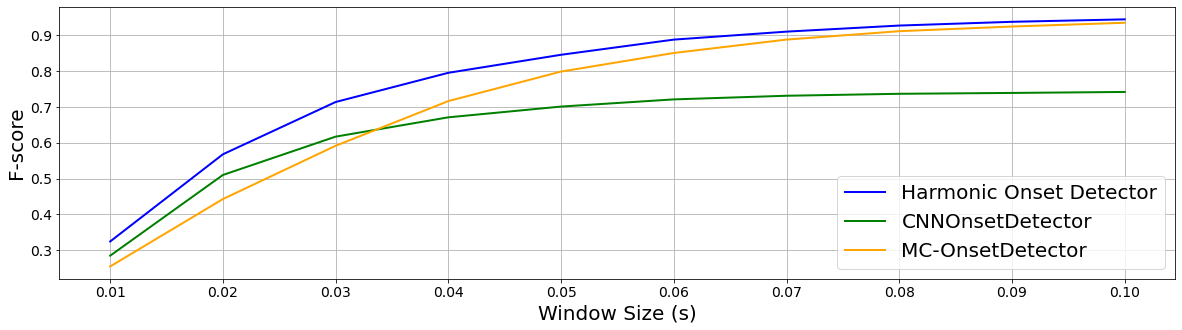
\includegraphics[width=\columnwidth]{results/mcwindowsize.png}
    \caption{F Scores of three onset detection algorithms on MusicCritic dataset w.r.t. size of tolerance window.}
    \label{fig:wsize_mc}
\end{figure}

\begin{figure}
    \centering
    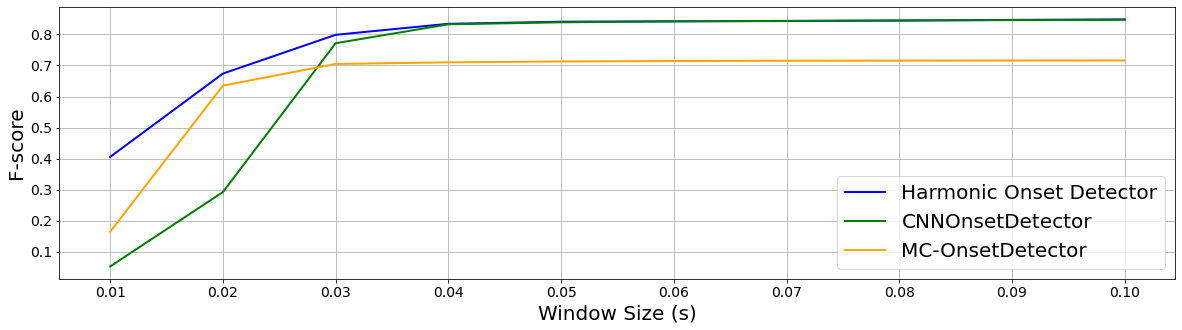
\includegraphics[width=\columnwidth]{results/gswindowsize.png}
    \caption{F Scores of three onset detection algorithms on GuitarSet data set w.r.t. size of tolerance window.}
    \label{fig:wsize_gs}
\end{figure}

\begin{table}
 \begin{center}
 \begin{tabular}{|l|l|l|l|}
  \hline
  & auto/human1 & auto/human2 & auto/humanAvg \\
  \hline
  Eremenko et al. \cite{eremenko2020performance} & 0.55 & 1.06 & 0.79\\
  MC-OnsetDetector & 0.36 & 0.76 & 0.43 \\
  CNNOnsetDetector & 0.43 & 0.98 & 0.56 \\
  Harmonic Onset Detector & 0.36 & 0.81 & 0.45 \\
  Ground truth onsets & 0.36 & 0.75 & 0.43 \\
  \hline
 \end{tabular}
\end{center}
 \caption{Mean Squared Error between grades given by human annotators and predicted grades}
 \label{tab:allassessment}
\end{table}

Onset detection results are converted to the onset difference deviations and automatic assessment experiments are conducted (Table \ref{tab:allassessment}). The first entry of the results is taken from the previous work, where MC-OnsetDetector was the algorithm used for onset detection. In the new result with the same algorithm (MC-OnsetDetector) the error is lower. The differences are the method of processing the onsets (see \ref{assessmethod}) and the recordings were trimmed when they have silences on the ends (see \ref{mc_annot}). MSE of the predictions is the lowest with MC-OnsetDetector with a 0.02 difference with Harmonic Onset Detector. MSE with the CNNOnsetDetector is higher than the other algorithms. Grade predictions did not improve when the ground truth onsets are used.  

\newpage

\chapter{Discussion}

\section{Results}

Harmonic Onset Detector had the highest score on average of two datasets. On GuitarSet, the algorithm performed poorly in two cases. First, if the duration between two onsets is less than the size of the smoothing window (148 ms), there is a chance of failure to detect both onsets, depending on the difference of energies introduced by those onsets and how close they are. Onsets closer than 148 ms are not common and they are not existent in MusicCritic dataset. Second, the algorithm does not detect dead notes\footnote{Dead notes are intentionally created percussive, non-pitched sounds.}. Dead notes are common on chord recordings of the GuitarSet and they are annotated as onsets. For this reason, the recall of the algorithm is low on chords (Table \ref{tab:threeGS}). On MusicCritic dataset, one limiting factor is the time accuracy. In chords, annotations are usually close to the middle of the strum, and the algorithm usually predicts the beginning of the strum as the onset. Due to strums generally being slow in this dataset, the predictions were not always inside the tolerance window. Scores of all three algorithms are increased continuously with the size of the tolerance window (Figure \ref{fig:wsize_mc}). Same effect was not observed in GuitarSet (Figure \ref{fig:wsize_gs}).  

MC-OnsetDetector algorithm applies two restrictions after the Superflux algorithm. It requires the RMS difference of two consecutive frames to be positive and spectral centroid to be smaller than a constant. These restrictions are found to be problematic and the reasons of low recall of the algorithm on GuitarSet. A glissando does not necessarily increase the energy, so can not be detected due to RMS difference restriction. Spectral centroid of the high frequency notes usually have larger spectral centroid than most of the noises, and the spectral centroid of a buzz noise can be even smaller than a low frequency note. These restrictions did not have the same detrimental effect on MusicCritic dataset. The first reason is, the RMS difference feature is useful against buzz noises (although buzz noises may increase the energy). Second, MusicCritic dataset does not contain many high frequency notes, which makes the spectral centroid a better feature to eliminate slide noises. In Figure \ref{fig:mc217}, the recording contains three distinct notes, F5 (698 Hz), G5 (783 Hz) and A5 (880 Hz). Due to the spectral centroid limitation, only the F5 notes are predicted correctly.  

CNNOnsetDetector obtained the highest recall and the lowest precision values on both datasets. It detects more onsets than other algorithms by a large margin, but it falsely predicts guitar noises as onsets too. Those false predictions are expected for two reasons. First, It is trained to detect various kinds of instruments. Noises in guitar recordings may have similar characteristics to onsets of other instruments (e.g. percussion instruments) in the training dataset of the neural network. Second, by tracking the information about the dataset in \cite{schluter2014improved} it can be assumed that the dataset which CNNOnsetDetector was trained does not contain any amateur guitar recordings. Therefore the neural network can not discriminate the guitar noises from guitar notes.

The algorithms are also evaluated on the guitar noises dataset. The dataset contains 36 buzz and 234 slide noises. The number of mistakes of the algorithms are; Harmonic Onset Detector 118 (29 buzz), MC-OnsetDetector 160 (5 buzz), CNNOnsetDetector 247 (29 buzz). These numbers do not represent the performance of algorithms in a realistic recording because (1) The noises of the dataset are intentionally exaggerated. (2) Some thresholds (e.g. for RMS, Spectral Flux) in algorithms depend on the existence of played notes in the audio (e.g. some slide noises are very quiet and eliminated by energy threshold). Harmonic Onset Detector performs quite poor on buzz noises for the following reasons: Buzz noises cause a decrease in frequency depending on the finger location (section \ref{buzzsection}) and the noises in the dataset are created by pressing the left side of the frets, which causes greater frequency decrease. Additionally, the player tried to keep the buzzing of the strings as long as possible. Since the algorithm seeks for new harmonic content for a long duration in a true onset, it fails on these extreme conditions of buzz noises. Such exaggerated buzz noises are only possible to find on performances of beginner players (e.g. when beginners try to play barre chords). The constant values of the algorithm can be adjusted to work better on beginner performances, which would make it worse on advanced performances. The automatic calculation of such constants could increase the overall performance of the algorithm.

Usage of the differences between the onsets decreased the MSE of the automatic rhythm assessment system (Table \ref{tab:allassessment}). MSE is higher with CNNOnsetDetector algorithm (Table \ref{tab:allassessment}), which can be explained with its poor performance on MusicCritic dataset (Table \ref{tab:threeMC}). Interestingly, ground truth onsets did not yield lower MSE than the onset predictions of Harmonic Onset Detector and MC-OnsetDetector, whose F-scores are 0.85 and 0.80. This result supports our argument in the onset processing method (see \ref{assessmethod}). The current onset detection evaluation can not distinguish between an algorithm that misses the tolerance window randomly and the one that misses consistently and we argued that each algorithm would be consistent even if they miss the tolerance window. The scores of Harmonic Onset Detector and MC-OnsetDetector are both increased to 0.95 when the tolerance window is increased from 50 ms to 100 ms (Figure \ref{fig:wsize_mc}), which showed that their predictions are mostly accurate but sometimes slightly out of the tolerance window. Their consistency can be seen in the example in Figure \ref{fig:hodmcod215}. Since the onset differences were similar for the ground truth onsets and both algorithms' onset predictions, the grade predictions were also similar. There are downsides of using only the onset differences. First, the average offset between notes and the metronome beats is lost (e.g. If all the notes are played late by same amount, the deviation of differences will be zero). Second, the differences between notes and metronome beats are needed for feedback to the students.


\section{Evaluation of Onset Detection}

In MIREX results\footnote{https://nema.lis.illinois.edu/nema\_out/mirex2018/results/aod/index.html}, the score of the CNNOnsetDetector on plucked strings category is reported as 0.90, which is significantly different than its scores in GuitarSet and MusicCritic dataset. For further examination, we evaluated the algorithm on MusicNet\footnote{MusicNet has a large amount of various classical music recordings. Nearly half of the recordings are solo piano (917 minutes), followed by string quartet (405 minutes)} \cite{thickstun}. F-score of CNNOnsetDetector is found to be 0.62 on MusicNet, which is again significantly lower than its reported scores on related categories (Complex: 0.82, Solo Sustained String: 0.77, Solo Winds: 0.78, Poly Pitched: 0.95). 

The difference between the scores of CNNOnsetDetector in our experiments and MIREX results raises concerns about the reliability of MIREX evaluations. The dataset used in MIREX evaluations (MIREX05 dataset\footnote{https://www.music-ir.org/mirex/wiki/2005:Audio\_Onset\_Detect}) contains only 14 minutes of recordings. It contains commercial recordings and excerpts from RWC database\footnote{https://staff.aist.go.jp/m.goto/RWC-MDB/}. This dataset may not be appropriate for accurate evaluations, thus fair comparisons of algorithms. There is a need of a new and larger test dataset for the onset detection task.

For the evaluations of onset detection algorithms in our work, the standard evaluation method was adopted at first. Then, we shifted the predicted onset values and changed the tolerance window sizes to understand the behaviour of the algorithms. Such plots were used for further clarification in some other studies too, e.g. \cite{holzapfel2009three}. This means that the standard evaluation method is not descriptive enough to make comparisons. When a framework for musical onset detection task is first introduced, it is assumed that a prediction should be classified as correct or false, and a prediction at time t is counted as correct if there exists a true onset within a time frame \([t - \tau, t + \tau]\) \cite{leveau2004}. The tolerance window (\(\tau\)) is later accepted as 50 ms \cite{bello2005tutorial}. According to this assumption, a prediction 50.1 ms away from a true onset is not different than the one 10 seconds away. Both of them are classified as false predictions, so making no prediction at all is considered to be better. For example, in Figure \ref{fig:hodmcod215}, if an algorithm correctly predicts 7 out of 16 chords and make no predictions for 9 remaining chords, it will achieve higher scores than the shown algorithms. This evaluation method does not explain well how an algorithm behaves, at least for our application. 

Onset detection is the first stage of many MIR applications and different applications naturally have different needs. An evaluation method that compares onset detection algorithms should provide useful information for all applications. For this purpose, metrics of the evaluation should fit the nature of the onset detection task. Classes, such as "true" and "false", implies the existence of distinctive qualities between things. There is no such quality that makes a prediction with 50 ms error true and but the one with 51 ms false, or all the predictions below 50 ms equally true and the ones above equally false. If we suggest a metric that depends on distances directly, instead of true-false classes, then we would need another threshold for matching predictions to ground truth onsets for the following reason: If we match the closest ground truth - predicted onset pairs without a threshold, the distance between a pair can be very large. For an algorithm that only uses, say, 100 ms around time instants to make predictions, a pair with a distance more than 100 ms does not make sense. In that case, the prediction should be classified as false, as it can not be associated with a ground truth onset. One option would be to set a threshold to define false predictions and use distance metrics to elaborate on true onsets. 


\begin{figure}
    \centering
    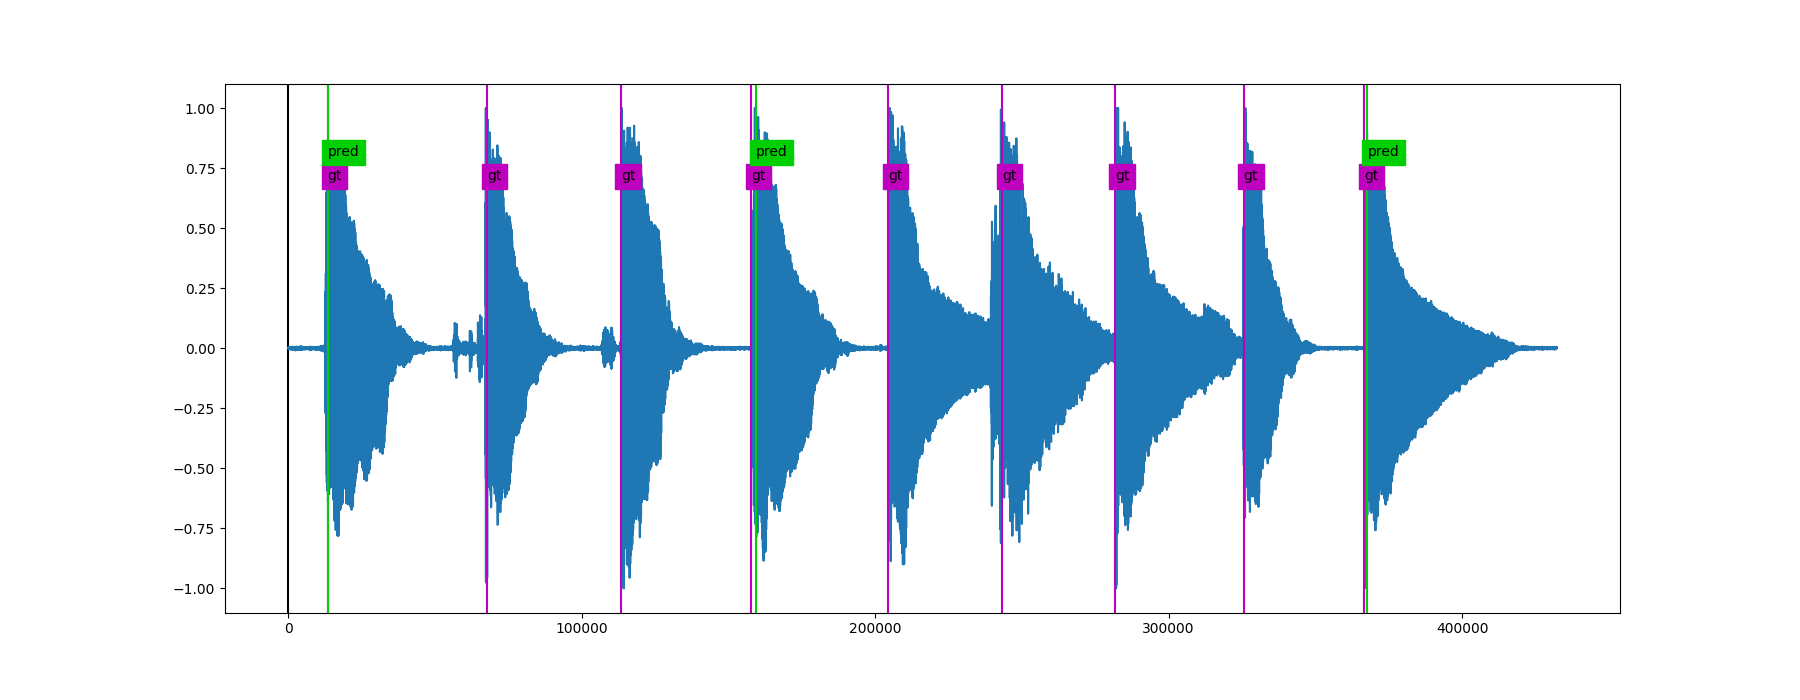
\includegraphics[width=\columnwidth]{discussion/MC217.png}
    \caption{Predictions of MC-OnsetDetector on a solo recording. Detected onsets are F5 notes. Undetected notes are G5 and A5. (Purple lines: ground truth onsets, Green lines: onset predictions)}
    \label{fig:mc217}
\end{figure}

\begin{figure}
    \centering
    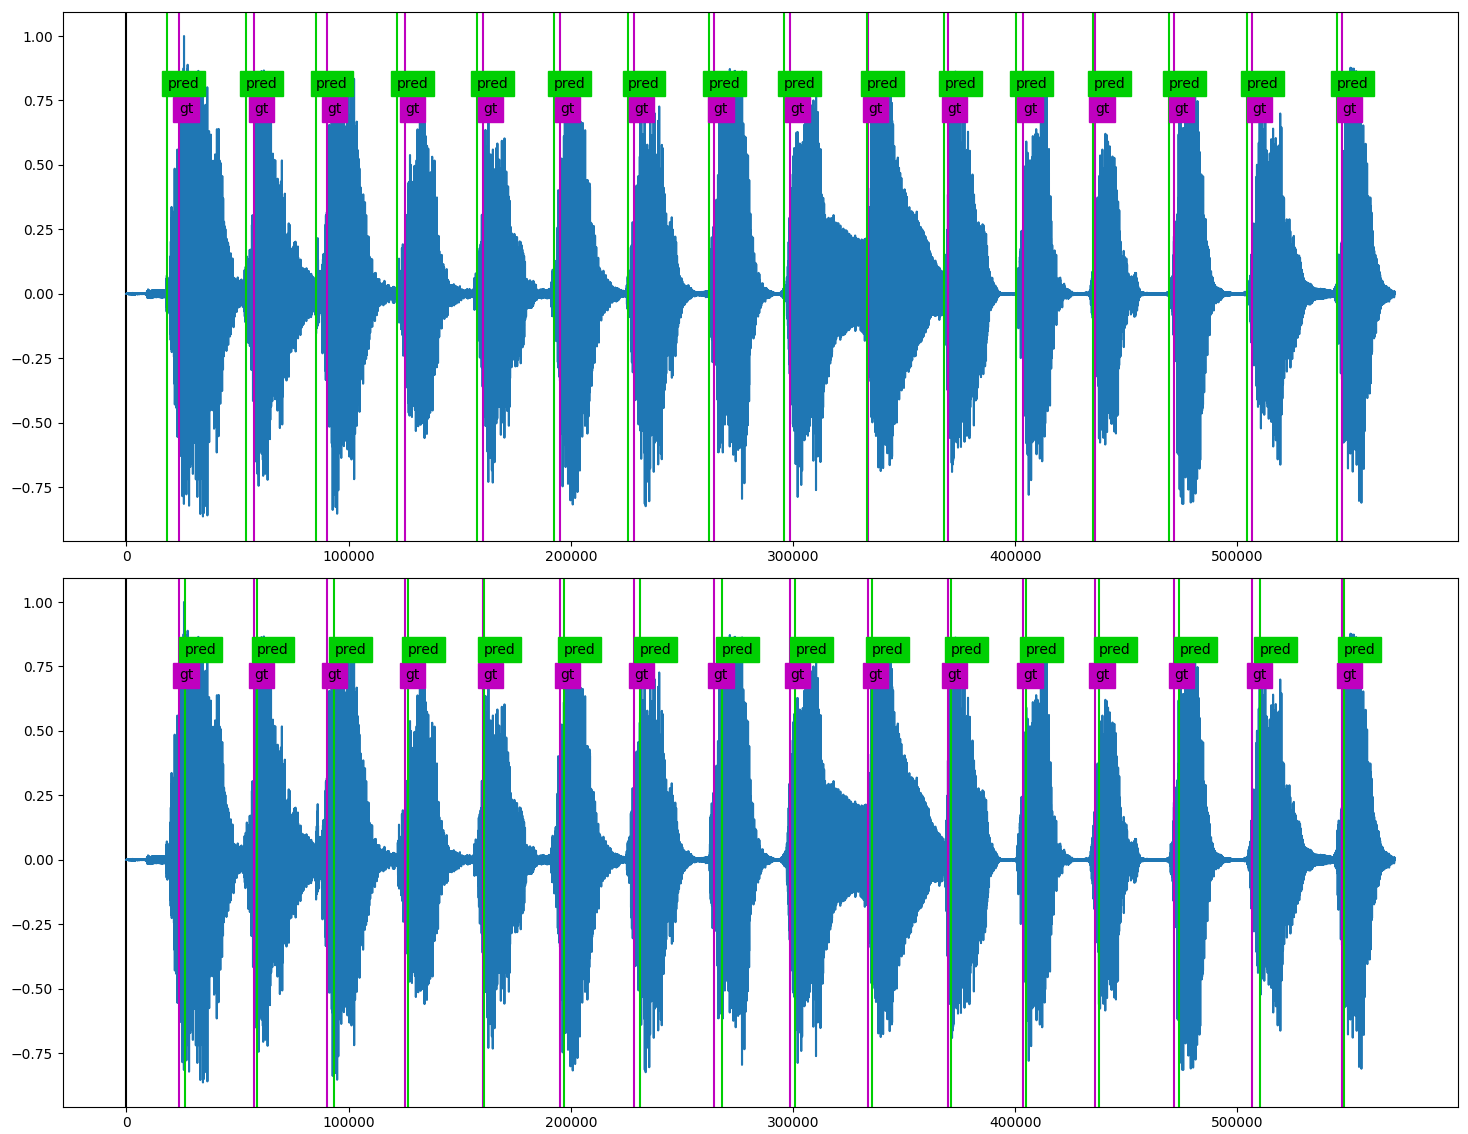
\includegraphics[width=\columnwidth]{discussion/hodmcod215.png}
    \caption{Predictions of Harmonic Onset Detector (top) and MC-OnsetDetector on a strummed chords. The algorithms aim at different locations of the chords. Due to long duration of the strums, some of the predictions are not accepted. F-scores are 0.44 and 0.55. (Purple lines: ground truth onsets, Green lines: onset predictions)}
    \label{fig:hodmcod215}
\end{figure}

\newpage



\chapter{Conclusion and Future Work}
In this work, our goal was to improve the onset detection for online guitar courses, where the recordings are amateur (noisy, reverberated etc.). We studied the common noises in amateur recordings and developed an algorithm to perform better in such recordings. We compared our algorithm, Harmonic Onset Detector, on three separate datasets (GuitarSet, MusicCritic, Guitar Noises) against the state-of-the-art algorithm (CNNOnsetDetector) and the algorithm of MusicCritic (MC-OnsetDetector). Algorithms were evaluated with different offset and threshold values. Overall, Harmonic Onset Detector was found to be robust against noises and better at detecting guitar notes in beginner exercises and realistic recordings. We improved the automatic rhythm assessment predictions of MusicCritic dataset and expressed the importance of onset detection in automatic assessment. During the course of the work, an annotation and analysis tool was developed and a dataset of guitar noises was created. Both are available online (see appendix).

Although the new algorithm is developed with a focus on guitars, it can be adjusted to other pitched instruments too. In an online course setting, some parameters of the algorithm can be adjusted automatically according to the exercise. These adjustments would improve performance further. For example, information of tempo and the shortest note duration can be used to adjust the total length threshold of the segmentation step. Some parameters (e.g. smoothing window size) have different optimal values for chords and single notes. In our evaluations, we used the same value for both chord and solo recordings, which was non-optimal for both. So the type of exercise could also be used. Downsides of the algorithm are (1) It is computationally more expensive than other algorithms. (2) A playing technique where the intended sound is percussive and non-pitched (dead note) is neglected.

In many studies (in the field of MIR), development and validation parts of datasets come from the same distribution, so the algorithms are often biased on the dataset they are evaluated. In our study, we also showed that performances of onset detection algorithms highly depend on the application and context. In literature, the onset detection task is sometimes considered solved, at least for percussive (pitched or non-pitched) instruments. Our results show that the task is far from solved. The algorithms only work on trivial recordings and fail on real life scenarios. The main reason is that the description of musical onsets changes with the context, and a human can adapt to it easily. For example, in a noisy environment, knowing which instruments are played helps a human to detect the musical notes. A human-level universal onset detection system would require a source separation and identification algorithms. Such algorithms would require large datasets for both evaluation or training. 

Currently, lack of available datasets (especially on music performance analysis) is a major obstacle in the development of both onset detection and automatic assessment algorithms. One solution is the data augmentation techniques, as it is used on other tasks such as sound classification \cite{salamon2017deep}. Noises that can occur in non-ideal recording environments can be added to existing onset detection datasets. Mathematical models of instrument specific noises can be used to generate artificial noises for data augmentation. For guitars, there are models for slide noises \cite{pakarinen2007analysis} but not for buzz noises. Methods used for sitar sound synthesis \cite{vyasarayani2009} can be adapted to guitars to generate buzz noises. 

The standard evaluation method of onset detection was not effective in describing the behaviours of algorithms, which was discussed in the previous chapter. There is a need for new evaluation methods or metrics for better explanation and comparison of the onset detection algorithms.

We discussed PATs (perceived attack times) of strummed chords in related work and automatic rhythm assessment sections. We used the subjectivity argument to use the onset to onset differences instead of onset to metronome differences in rhythm assessment. For more accurate rhythm assessment and feedback, we still need to predict PATs of strummed chords. More studies with listening experiments are needed in order to develop a PAT prediction model. 

\newpage


\listoffigures
\newpage
\listoftables

% appendices come here
\bibliographystyle{naturemag}
\bibliography{bibliography}

\appendix
\chapter{Sound Annotation and Analysis Tool}\label{appendix:a} %Appendix

\begin{figure}
    \centering
    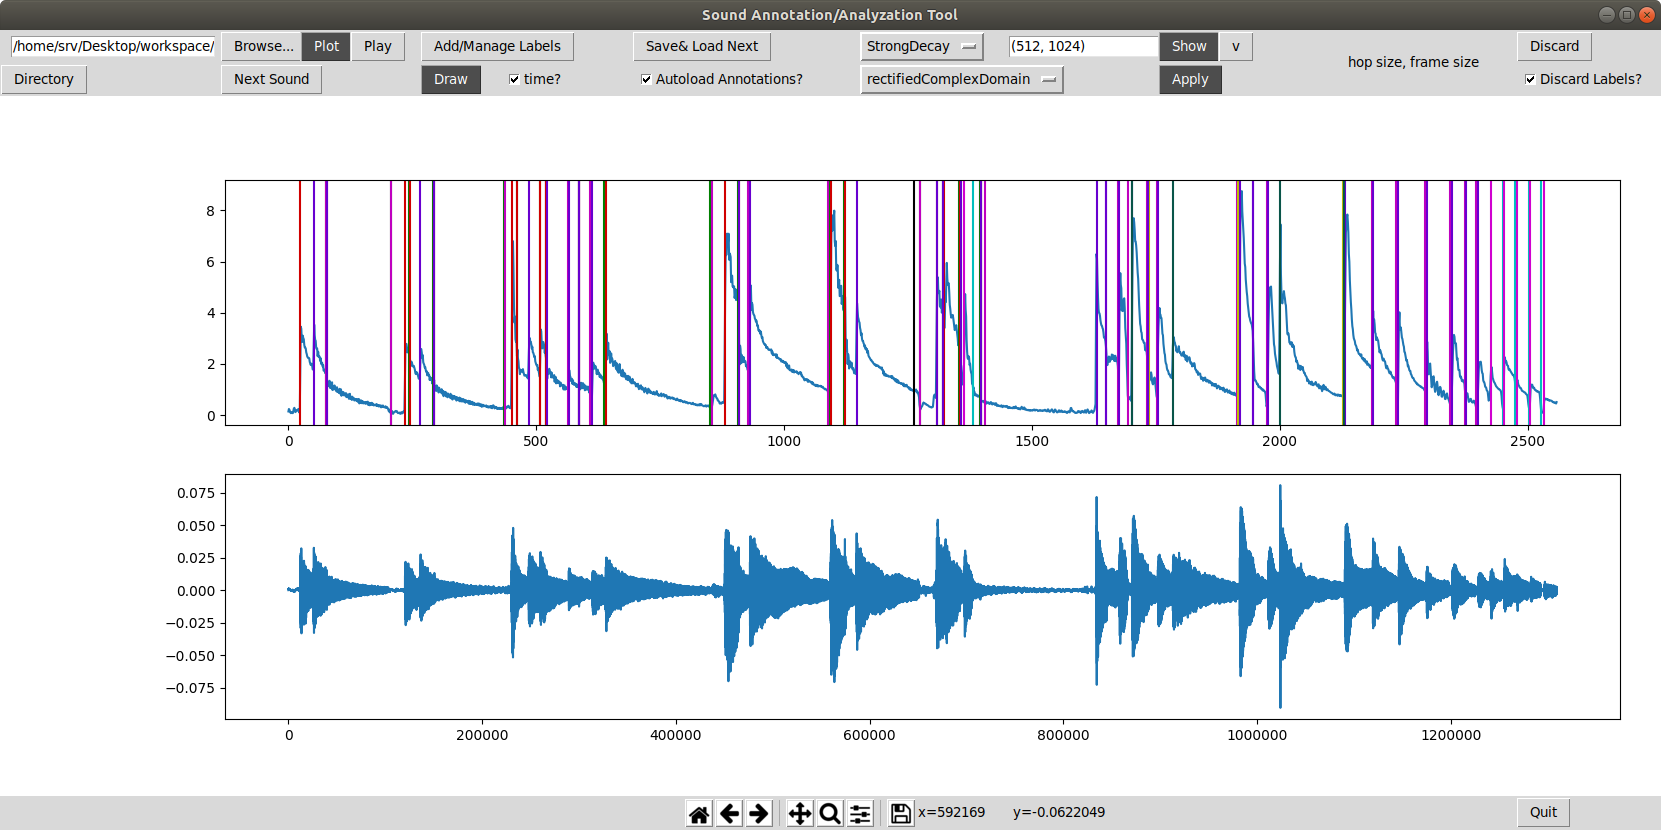
\includegraphics[width=\columnwidth]{appendix/saat.png}
    \caption{A screenshot of the Sound Annotation and Analysis Tool}
    \label{fig:saat}
\end{figure}

This tool is developed to save time on annotation and inspection of the sound files. Written in Python.

GUI: Tkinter (https://docs.python.org/3/library/tkinter.html)\\
Sound: PyAudio (https://pypi.org/project/PyAudio/)\\
Audio Features: Essentia (https://essentia.upf.edu/)\\
Onset Detection Functions: Essentia and madmom (https://pypi.org/project/madmom/)\\

Audio features from Essentia library can be extracted and plotted on the interactive frame. Interactive frame allows navigation through the plot and control the sound player. Two features can be shown at the same time. 
Onset detection functions from Essentia and madmom library can be applied to the loaded sound. Detected onsets can be saved as annotations.

\newpage

\chapter{Guitar Noises Dataset}\label{appendix:b}

Dataset is available on https://freesound.org/people/svurucu/packs/29986/.

Buzz noises are created via following procedure: String is pressed on the left side of the fret (closer to headstock) and the note is played naturally by plucking the string. Then, the string is slowly released until it produce a buzz (see \ref{buzzsection}).  \\

Slide noises are generated between two predetermined frets. The player had one second to move between each origin-destination fret pairs. Movement had to start and end inside of the one second duration. Slide noises have two versions, the string can be released or still pressed at the beginning of the slide. The latter causes a louder 'squeak' sound. Origin-destination fret pairs are selected by fixing the origin, or their distance. Then, all possible combinations are performed within the first twelve frets.

Currently, there are 36 buzz and 234 slide noises available.

\textbf{Recording Details:}

Guitar: Yamaha C80 Classical Guitar \\
Strings: D'Addario EXP45 Coated Classical Guitar Strings, Normal Tension \\
Microphone: Samson C05 (The microphone was placed 10 cm in front of the sound hole)\\
Soundcard: Focusrite Scarlett 18i20 \\
Environment: Small (6m$^2$) anechoic chamber \\

\end{document}
